% Options for packages loaded elsewhere
\PassOptionsToPackage{unicode}{hyperref}
\PassOptionsToPackage{hyphens}{url}
\PassOptionsToPackage{dvipsnames,svgnames,x11names}{xcolor}
%
\documentclass[
  letterpaper,
  DIV=11,
  numbers=noendperiod,
  oneside]{scrreprt}

\usepackage{amsmath,amssymb}
\usepackage{iftex}
\ifPDFTeX
  \usepackage[T1]{fontenc}
  \usepackage[utf8]{inputenc}
  \usepackage{textcomp} % provide euro and other symbols
\else % if luatex or xetex
  \usepackage{unicode-math}
  \defaultfontfeatures{Scale=MatchLowercase}
  \defaultfontfeatures[\rmfamily]{Ligatures=TeX,Scale=1}
\fi
\usepackage{lmodern}
\ifPDFTeX\else  
    % xetex/luatex font selection
\fi
% Use upquote if available, for straight quotes in verbatim environments
\IfFileExists{upquote.sty}{\usepackage{upquote}}{}
\IfFileExists{microtype.sty}{% use microtype if available
  \usepackage[]{microtype}
  \UseMicrotypeSet[protrusion]{basicmath} % disable protrusion for tt fonts
}{}
\makeatletter
\@ifundefined{KOMAClassName}{% if non-KOMA class
  \IfFileExists{parskip.sty}{%
    \usepackage{parskip}
  }{% else
    \setlength{\parindent}{0pt}
    \setlength{\parskip}{6pt plus 2pt minus 1pt}}
}{% if KOMA class
  \KOMAoptions{parskip=half}}
\makeatother
\usepackage{xcolor}
\usepackage[left=1in,marginparwidth=2.0666666666667in,textwidth=4.1333333333333in,marginparsep=0.3in]{geometry}
\setlength{\emergencystretch}{3em} % prevent overfull lines
\setcounter{secnumdepth}{5}
% Make \paragraph and \subparagraph free-standing
\makeatletter
\ifx\paragraph\undefined\else
  \let\oldparagraph\paragraph
  \renewcommand{\paragraph}{
    \@ifstar
      \xxxParagraphStar
      \xxxParagraphNoStar
  }
  \newcommand{\xxxParagraphStar}[1]{\oldparagraph*{#1}\mbox{}}
  \newcommand{\xxxParagraphNoStar}[1]{\oldparagraph{#1}\mbox{}}
\fi
\ifx\subparagraph\undefined\else
  \let\oldsubparagraph\subparagraph
  \renewcommand{\subparagraph}{
    \@ifstar
      \xxxSubParagraphStar
      \xxxSubParagraphNoStar
  }
  \newcommand{\xxxSubParagraphStar}[1]{\oldsubparagraph*{#1}\mbox{}}
  \newcommand{\xxxSubParagraphNoStar}[1]{\oldsubparagraph{#1}\mbox{}}
\fi
\makeatother

\usepackage{color}
\usepackage{fancyvrb}
\newcommand{\VerbBar}{|}
\newcommand{\VERB}{\Verb[commandchars=\\\{\}]}
\DefineVerbatimEnvironment{Highlighting}{Verbatim}{commandchars=\\\{\}}
% Add ',fontsize=\small' for more characters per line
\usepackage{framed}
\definecolor{shadecolor}{RGB}{241,243,245}
\newenvironment{Shaded}{\begin{snugshade}}{\end{snugshade}}
\newcommand{\AlertTok}[1]{\textcolor[rgb]{0.68,0.00,0.00}{#1}}
\newcommand{\AnnotationTok}[1]{\textcolor[rgb]{0.37,0.37,0.37}{#1}}
\newcommand{\AttributeTok}[1]{\textcolor[rgb]{0.40,0.45,0.13}{#1}}
\newcommand{\BaseNTok}[1]{\textcolor[rgb]{0.68,0.00,0.00}{#1}}
\newcommand{\BuiltInTok}[1]{\textcolor[rgb]{0.00,0.23,0.31}{#1}}
\newcommand{\CharTok}[1]{\textcolor[rgb]{0.13,0.47,0.30}{#1}}
\newcommand{\CommentTok}[1]{\textcolor[rgb]{0.37,0.37,0.37}{#1}}
\newcommand{\CommentVarTok}[1]{\textcolor[rgb]{0.37,0.37,0.37}{\textit{#1}}}
\newcommand{\ConstantTok}[1]{\textcolor[rgb]{0.56,0.35,0.01}{#1}}
\newcommand{\ControlFlowTok}[1]{\textcolor[rgb]{0.00,0.23,0.31}{\textbf{#1}}}
\newcommand{\DataTypeTok}[1]{\textcolor[rgb]{0.68,0.00,0.00}{#1}}
\newcommand{\DecValTok}[1]{\textcolor[rgb]{0.68,0.00,0.00}{#1}}
\newcommand{\DocumentationTok}[1]{\textcolor[rgb]{0.37,0.37,0.37}{\textit{#1}}}
\newcommand{\ErrorTok}[1]{\textcolor[rgb]{0.68,0.00,0.00}{#1}}
\newcommand{\ExtensionTok}[1]{\textcolor[rgb]{0.00,0.23,0.31}{#1}}
\newcommand{\FloatTok}[1]{\textcolor[rgb]{0.68,0.00,0.00}{#1}}
\newcommand{\FunctionTok}[1]{\textcolor[rgb]{0.28,0.35,0.67}{#1}}
\newcommand{\ImportTok}[1]{\textcolor[rgb]{0.00,0.46,0.62}{#1}}
\newcommand{\InformationTok}[1]{\textcolor[rgb]{0.37,0.37,0.37}{#1}}
\newcommand{\KeywordTok}[1]{\textcolor[rgb]{0.00,0.23,0.31}{\textbf{#1}}}
\newcommand{\NormalTok}[1]{\textcolor[rgb]{0.00,0.23,0.31}{#1}}
\newcommand{\OperatorTok}[1]{\textcolor[rgb]{0.37,0.37,0.37}{#1}}
\newcommand{\OtherTok}[1]{\textcolor[rgb]{0.00,0.23,0.31}{#1}}
\newcommand{\PreprocessorTok}[1]{\textcolor[rgb]{0.68,0.00,0.00}{#1}}
\newcommand{\RegionMarkerTok}[1]{\textcolor[rgb]{0.00,0.23,0.31}{#1}}
\newcommand{\SpecialCharTok}[1]{\textcolor[rgb]{0.37,0.37,0.37}{#1}}
\newcommand{\SpecialStringTok}[1]{\textcolor[rgb]{0.13,0.47,0.30}{#1}}
\newcommand{\StringTok}[1]{\textcolor[rgb]{0.13,0.47,0.30}{#1}}
\newcommand{\VariableTok}[1]{\textcolor[rgb]{0.07,0.07,0.07}{#1}}
\newcommand{\VerbatimStringTok}[1]{\textcolor[rgb]{0.13,0.47,0.30}{#1}}
\newcommand{\WarningTok}[1]{\textcolor[rgb]{0.37,0.37,0.37}{\textit{#1}}}

\providecommand{\tightlist}{%
  \setlength{\itemsep}{0pt}\setlength{\parskip}{0pt}}\usepackage{longtable,booktabs,array}
\usepackage{calc} % for calculating minipage widths
% Correct order of tables after \paragraph or \subparagraph
\usepackage{etoolbox}
\makeatletter
\patchcmd\longtable{\par}{\if@noskipsec\mbox{}\fi\par}{}{}
\makeatother
% Allow footnotes in longtable head/foot
\IfFileExists{footnotehyper.sty}{\usepackage{footnotehyper}}{\usepackage{footnote}}
\makesavenoteenv{longtable}
\usepackage{graphicx}
\makeatletter
\def\maxwidth{\ifdim\Gin@nat@width>\linewidth\linewidth\else\Gin@nat@width\fi}
\def\maxheight{\ifdim\Gin@nat@height>\textheight\textheight\else\Gin@nat@height\fi}
\makeatother
% Scale images if necessary, so that they will not overflow the page
% margins by default, and it is still possible to overwrite the defaults
% using explicit options in \includegraphics[width, height, ...]{}
\setkeys{Gin}{width=\maxwidth,height=\maxheight,keepaspectratio}
% Set default figure placement to htbp
\makeatletter
\def\fps@figure{htbp}
\makeatother

\KOMAoption{captions}{tableheading}
\makeatletter
\@ifpackageloaded{tcolorbox}{}{\usepackage[skins,breakable]{tcolorbox}}
\@ifpackageloaded{fontawesome5}{}{\usepackage{fontawesome5}}
\definecolor{quarto-callout-color}{HTML}{909090}
\definecolor{quarto-callout-note-color}{HTML}{0758E5}
\definecolor{quarto-callout-important-color}{HTML}{CC1914}
\definecolor{quarto-callout-warning-color}{HTML}{EB9113}
\definecolor{quarto-callout-tip-color}{HTML}{00A047}
\definecolor{quarto-callout-caution-color}{HTML}{FC5300}
\definecolor{quarto-callout-color-frame}{HTML}{acacac}
\definecolor{quarto-callout-note-color-frame}{HTML}{4582ec}
\definecolor{quarto-callout-important-color-frame}{HTML}{d9534f}
\definecolor{quarto-callout-warning-color-frame}{HTML}{f0ad4e}
\definecolor{quarto-callout-tip-color-frame}{HTML}{02b875}
\definecolor{quarto-callout-caution-color-frame}{HTML}{fd7e14}
\makeatother
\makeatletter
\@ifpackageloaded{caption}{}{\usepackage{caption}}
\AtBeginDocument{%
\ifdefined\contentsname
  \renewcommand*\contentsname{Table of contents}
\else
  \newcommand\contentsname{Table of contents}
\fi
\ifdefined\listfigurename
  \renewcommand*\listfigurename{List of Figures}
\else
  \newcommand\listfigurename{List of Figures}
\fi
\ifdefined\listtablename
  \renewcommand*\listtablename{List of Tables}
\else
  \newcommand\listtablename{List of Tables}
\fi
\ifdefined\figurename
  \renewcommand*\figurename{Figure}
\else
  \newcommand\figurename{Figure}
\fi
\ifdefined\tablename
  \renewcommand*\tablename{Table}
\else
  \newcommand\tablename{Table}
\fi
}
\@ifpackageloaded{float}{}{\usepackage{float}}
\floatstyle{ruled}
\@ifundefined{c@chapter}{\newfloat{codelisting}{h}{lop}}{\newfloat{codelisting}{h}{lop}[chapter]}
\floatname{codelisting}{Listing}
\newcommand*\listoflistings{\listof{codelisting}{List of Listings}}
\makeatother
\makeatletter
\makeatother
\makeatletter
\@ifpackageloaded{caption}{}{\usepackage{caption}}
\@ifpackageloaded{subcaption}{}{\usepackage{subcaption}}
\makeatother
\makeatletter
\@ifpackageloaded{sidenotes}{}{\usepackage{sidenotes}}
\@ifpackageloaded{marginnote}{}{\usepackage{marginnote}}
\makeatother

\ifLuaTeX
  \usepackage{selnolig}  % disable illegal ligatures
\fi
\usepackage{bookmark}

\IfFileExists{xurl.sty}{\usepackage{xurl}}{} % add URL line breaks if available
\urlstyle{same} % disable monospaced font for URLs
\hypersetup{
  pdftitle={Mapping},
  pdfauthor={Andrew Grogan-Kaylor},
  colorlinks=true,
  linkcolor={blue},
  filecolor={Maroon},
  citecolor={Blue},
  urlcolor={Blue},
  pdfcreator={LaTeX via pandoc}}


\title{Mapping}
\usepackage{etoolbox}
\makeatletter
\providecommand{\subtitle}[1]{% add subtitle to \maketitle
  \apptocmd{\@title}{\par {\large #1 \par}}{}{}
}
\makeatother
\subtitle{Materials for an \emph{In Development} Course on GIS \&
Mapping}
\author{Andrew Grogan-Kaylor}
\date{2024-11-23}

\begin{document}
\maketitle

\renewcommand*\contentsname{Table of contents}
{
\hypersetup{linkcolor=}
\setcounter{tocdepth}{2}
\tableofcontents
}
\listoffigures
\listoftables

\chapter{Introduction to Mapping and
GIS}\label{introduction-to-mapping-and-gis}

\begin{figure}

\centering{

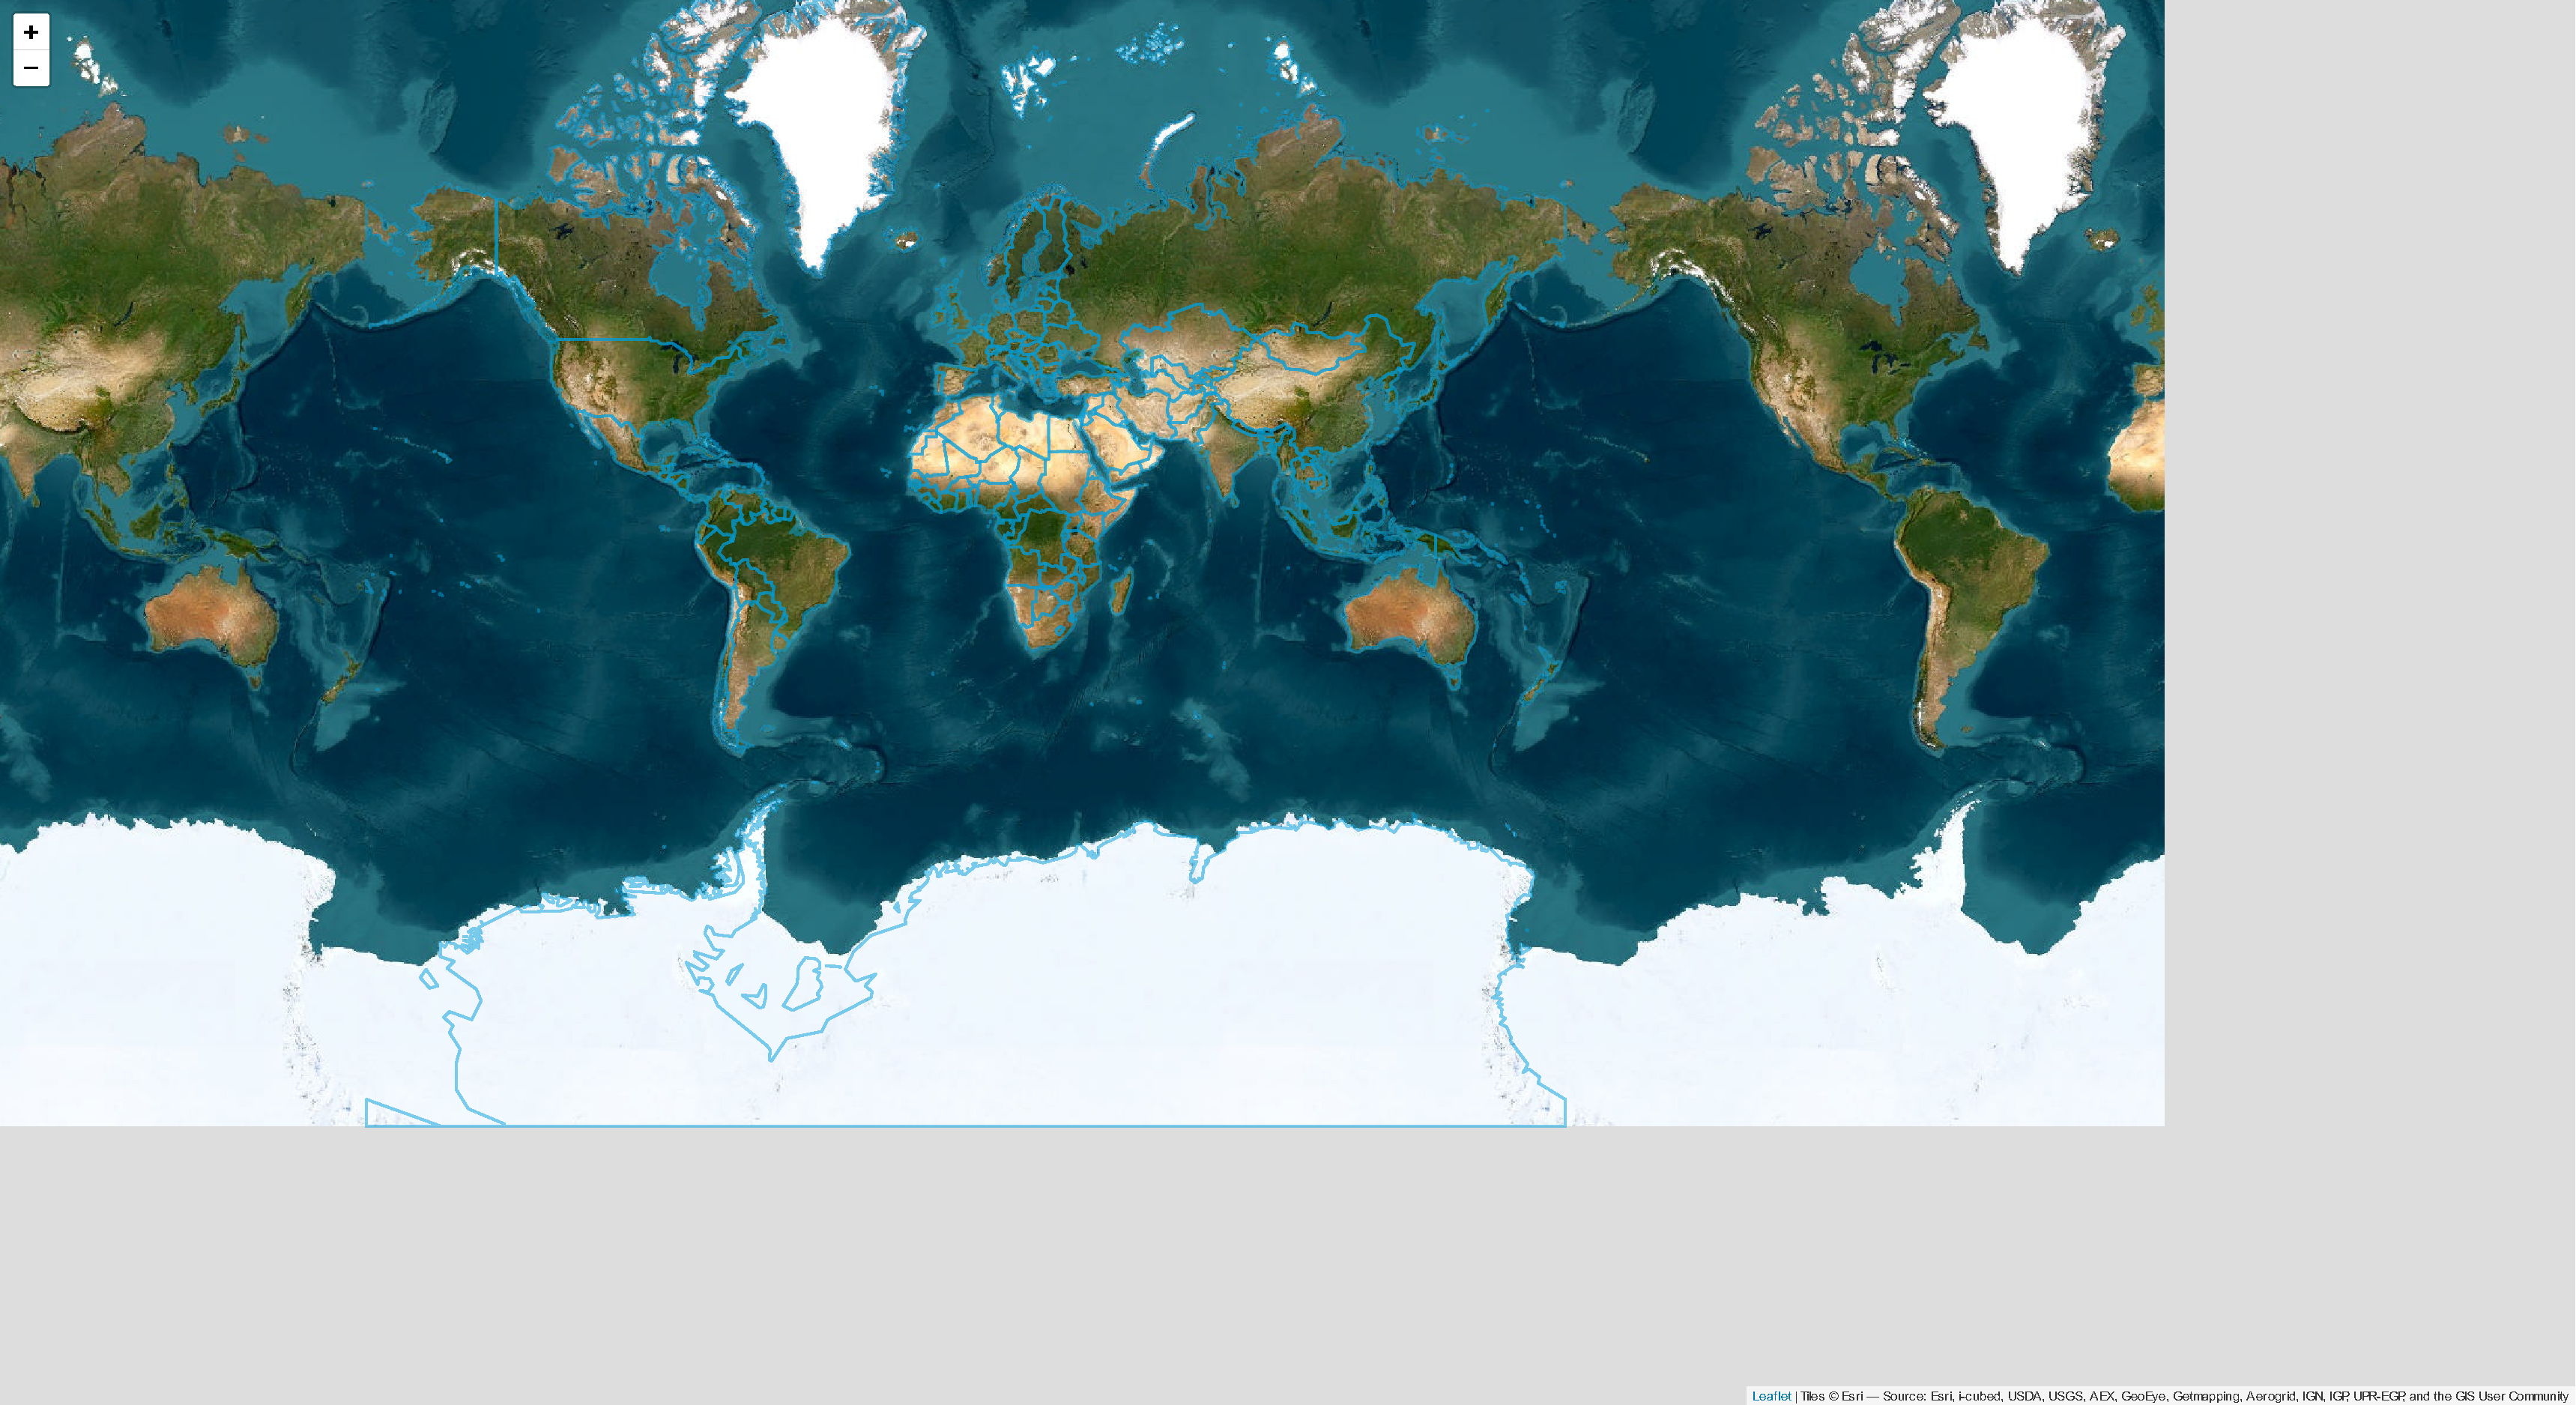
\includegraphics{index_files/figure-pdf/fig-world-1.pdf}

}

\caption{\label{fig-world}Countries of the World}

\end{figure}%

Mapping and GIS have become an increasingly important part of social
research, advocacy, and program and policy development. This website
contains materials for an \emph{in development} course on \emph{Mapping
and GIS}.

The content of this site is built around the use of R software, though
many of the concepts are applicable across GIS and mapping applications
such as R, Stata, ArcGIS and QGIS.

\part{Introduction}

\chapter{Possible Course Outline}\label{possible-course-outline}

\begin{tcolorbox}[enhanced jigsaw, opacityback=0, colback=white, toprule=.15mm, colframe=quarto-callout-important-color-frame, bottomrule=.15mm, title=\textcolor{quarto-callout-important-color}{\faExclamation}\hspace{0.5em}{Mapping is FUN \textbf{and} CHALLENGING}, coltitle=black, toptitle=1mm, bottomtitle=1mm, arc=.35mm, breakable, colbacktitle=quarto-callout-important-color!10!white, left=2mm, rightrule=.15mm, titlerule=0mm, leftrule=.75mm, opacitybacktitle=0.6]

Mapping is fun. Many people enjoy looking at maps, and find them
informative and helpful. Many people find it very fun to learn how to
make maps. At the same time, making even basic maps with geographic data
can be challenging. Making an aesthetically pleasing and useful map can
be very challenging. We will work hard in this course to learn these
important skills. At the same time, we will have fun doing so!

\end{tcolorbox}

\section{5 Week MiniCourse}\label{sec-fiveweek}

\begin{enumerate}
\def\labelenumi{\arabic{enumi}.}
\tightlist
\item
  Introduction

  \begin{itemize}
  \tightlist
  \item
    Introduction to the Course
  \item
    Introduction to Shapefiles (and Possibly \texttt{sf} Objects) As GIS
    Data
  \item
    Introduction to Appropriate Software: R / RStudio / \texttt{sf} /
    \texttt{ggplot}; or ArcGIS; or QGIS; or Tableau
  \item
    Quick Mapping Exercise
  \end{itemize}
\item
  Basic GIS Skills

  \begin{itemize}
  \tightlist
  \item
    Symbology
  \item
    Joining by Attribute
  \end{itemize}
\item
  Data With Geographic Coordinates \& Geographic Concepts

  \begin{itemize}
  \tightlist
  \item
    Data With Latitude and Longitude
  \item
    Coordinate Reference Systems
  \end{itemize}
\item
  Geocoding
\item
  Lab Day for Final Projects
\end{enumerate}

\section{More Advanced Topics}\label{sec-moreadvanced}

\begin{enumerate}
\def\labelenumi{\arabic{enumi}.}
\tightlist
\item
  Basemaps e.g.~\texttt{leaflet} (Chapter~\ref{sec-leaflet})
\item
  Projections, projecting and re-projecting geographic data
  (Chapter~\ref{sec-projections})
\item
  Geoprocessing (Spatial joins; Spatial Selection; Selection by
  Attribute)
\end{enumerate}

\section{Full Semester Course}\label{full-semester-course}

\begin{itemize}
\tightlist
\item
  Begin with a coding (R) approach to the topics listed in
  Section~\ref{sec-fiveweek}.
\item
  Revisit these topics, and discuss each topic in more depth, with drag
  and drop software: ArcGIS; QGIS; Tableau. Build in more advanced
  topics (Section~\ref{sec-moreadvanced}).
\item
  Finish up with a \emph{Mapping Showcase} constructing useful maps with
  aesthetically pleasing and clearly understandable design elements.
\end{itemize}

\chapter{Introduction to R}\label{introduction-to-r}

\begin{itemize}
\tightlist
\item
  Introductory content on R can be found here:
  \url{https://globalfamilies.quarto.pub/global-families-project/quick-intro-R.html}.
\item
  Introductory content on ggplot for graphing and data visualization can
  be found here:
  \url{https://globalfamilies.quarto.pub/global-families-project/quick-intro-ggplot2.html}.
\end{itemize}

\part{Geographical and GIS Concepts}

\chapter{Latitude and Longitude}\label{latitude-and-longitude}

\section{Introduction}\label{introduction-1}

Latitude and longitude are coordinates for locating objects on earth.

\begin{itemize}
\tightlist
\item
  Latitude represents distance from the \emph{equator}.

  \begin{itemize}
  \tightlist
  \item
    0 latitude is at the equator.
  \item
    +90 latitude, or 90N, is at the North Pole.
  \item
    -90 latitude, or 90S, is at the South Pole.
  \end{itemize}
\item
  Longitude represents distance from the \emph{prime meridian}.

  \begin{itemize}
  \tightlist
  \item
    0 longitude is at the prime meridian.
  \item
    +180 and -180, or 180E and 180W, meet at the other side of the
    world.
  \end{itemize}
\end{itemize}

\section{Call the Libraries}\label{call-the-libraries}

\begin{Shaded}
\begin{Highlighting}[]
\FunctionTok{library}\NormalTok{(plotly)}
\end{Highlighting}
\end{Shaded}

\section{Generate Some Random
Coordinates}\label{generate-some-random-coordinates}

\begin{Shaded}
\begin{Highlighting}[]
\FunctionTok{set.seed}\NormalTok{(}\DecValTok{3846}\NormalTok{) }\CommentTok{\# random seed}

\NormalTok{N }\OtherTok{\textless{}{-}} \DecValTok{10} \CommentTok{\# number of points}

\CommentTok{\# latitude from {-}90 to +90}

\NormalTok{latitude }\OtherTok{\textless{}{-}} \FunctionTok{runif}\NormalTok{(N, }\AttributeTok{min =} \SpecialCharTok{{-}}\DecValTok{90}\NormalTok{, }\AttributeTok{max =} \DecValTok{90}\NormalTok{) }

\CommentTok{\# longitude from + {-}180 to + 180}

\NormalTok{longitude }\OtherTok{\textless{}{-}} \FunctionTok{runif}\NormalTok{(N, }\AttributeTok{min =} \SpecialCharTok{{-}}\DecValTok{180}\NormalTok{, }\AttributeTok{max =} \DecValTok{180}\NormalTok{) }

\CommentTok{\# 1st point reset to 0, 0}

\NormalTok{latitude[}\DecValTok{1}\NormalTok{] }\OtherTok{\textless{}{-}} \DecValTok{0} \CommentTok{\# equator}

\NormalTok{longitude[}\DecValTok{1}\NormalTok{] }\OtherTok{\textless{}{-}} \DecValTok{0} \CommentTok{\# prime meridian}

\NormalTok{latitude[}\DecValTok{2}\NormalTok{] }\OtherTok{\textless{}{-}} \DecValTok{42} \CommentTok{\# Ann Arbor{-}ish}

\NormalTok{longitude[}\DecValTok{2}\NormalTok{] }\OtherTok{\textless{}{-}} \SpecialCharTok{{-}}\FloatTok{83.5} \CommentTok{\# Ann Arbor{-}ish}

\CommentTok{\# label}

\NormalTok{label }\OtherTok{\textless{}{-}}\NormalTok{ LETTERS[}\DecValTok{1}\SpecialCharTok{:}\NormalTok{N] }\CommentTok{\# label with letters of alphabet}

\CommentTok{\# dataframe}

\NormalTok{mydata }\OtherTok{\textless{}{-}} \FunctionTok{data.frame}\NormalTok{(latitude, longitude, label)}

\NormalTok{mydata }\CommentTok{\# replay}
\end{Highlighting}
\end{Shaded}

\begin{verbatim}
     latitude  longitude label
1    0.000000    0.00000     A
2   42.000000  -83.50000     B
3    7.023357   73.49444     C
4  -38.775631  159.53317     D
5  -80.547165 -129.12572     E
6  -17.472905   25.95547     F
7  -69.826706  -54.36372     G
8   10.498416   14.20623     H
9  -72.440487  -27.65036     I
10 -46.753424  130.83572     J
\end{verbatim}

\section{Map The Coordinates}\label{map-the-coordinates}

\begin{Shaded}
\begin{Highlighting}[]
\NormalTok{g }\OtherTok{\textless{}{-}} \FunctionTok{list}\NormalTok{(}\AttributeTok{lonaxis =} \FunctionTok{list}\NormalTok{(}\AttributeTok{showgrid =}\NormalTok{ T, }\CommentTok{\# geographic parameters}
                         \AttributeTok{gridcolor =} \StringTok{"lightblue"}\NormalTok{), }
          \AttributeTok{lataxis =} \FunctionTok{list}\NormalTok{(}\AttributeTok{showgrid =}\NormalTok{ T, }
                         \AttributeTok{gridcolor =} \StringTok{"lightblue"}\NormalTok{),}
          \AttributeTok{showland =} \ConstantTok{TRUE}\NormalTok{,}
          \AttributeTok{landcolor =} \FunctionTok{toRGB}\NormalTok{(}\StringTok{"lightgrey"}\NormalTok{))}

\NormalTok{mymap }\OtherTok{\textless{}{-}} \FunctionTok{plot\_geo}\NormalTok{(mydata) }\SpecialCharTok{\%\textgreater{}\%}
  \FunctionTok{add\_markers}\NormalTok{(}\AttributeTok{x =} \SpecialCharTok{\textasciitilde{}}\NormalTok{longitude,}
              \AttributeTok{y =} \SpecialCharTok{\textasciitilde{}}\NormalTok{latitude,}
              \AttributeTok{color =} \SpecialCharTok{\textasciitilde{}}\NormalTok{label,}
              \AttributeTok{colors =} \StringTok{"Spectral"}\NormalTok{,}
              \AttributeTok{marker =} \FunctionTok{list}\NormalTok{(}\AttributeTok{size =} \DecValTok{15}\NormalTok{)) }\SpecialCharTok{\%\textgreater{}\%}
  \FunctionTok{layout}\NormalTok{(}\AttributeTok{title =} \StringTok{"Randomly Generated Coordinates"}\NormalTok{,}
         \AttributeTok{geo =}\NormalTok{ g)}

\NormalTok{mymap }\CommentTok{\# replay}
\end{Highlighting}
\end{Shaded}

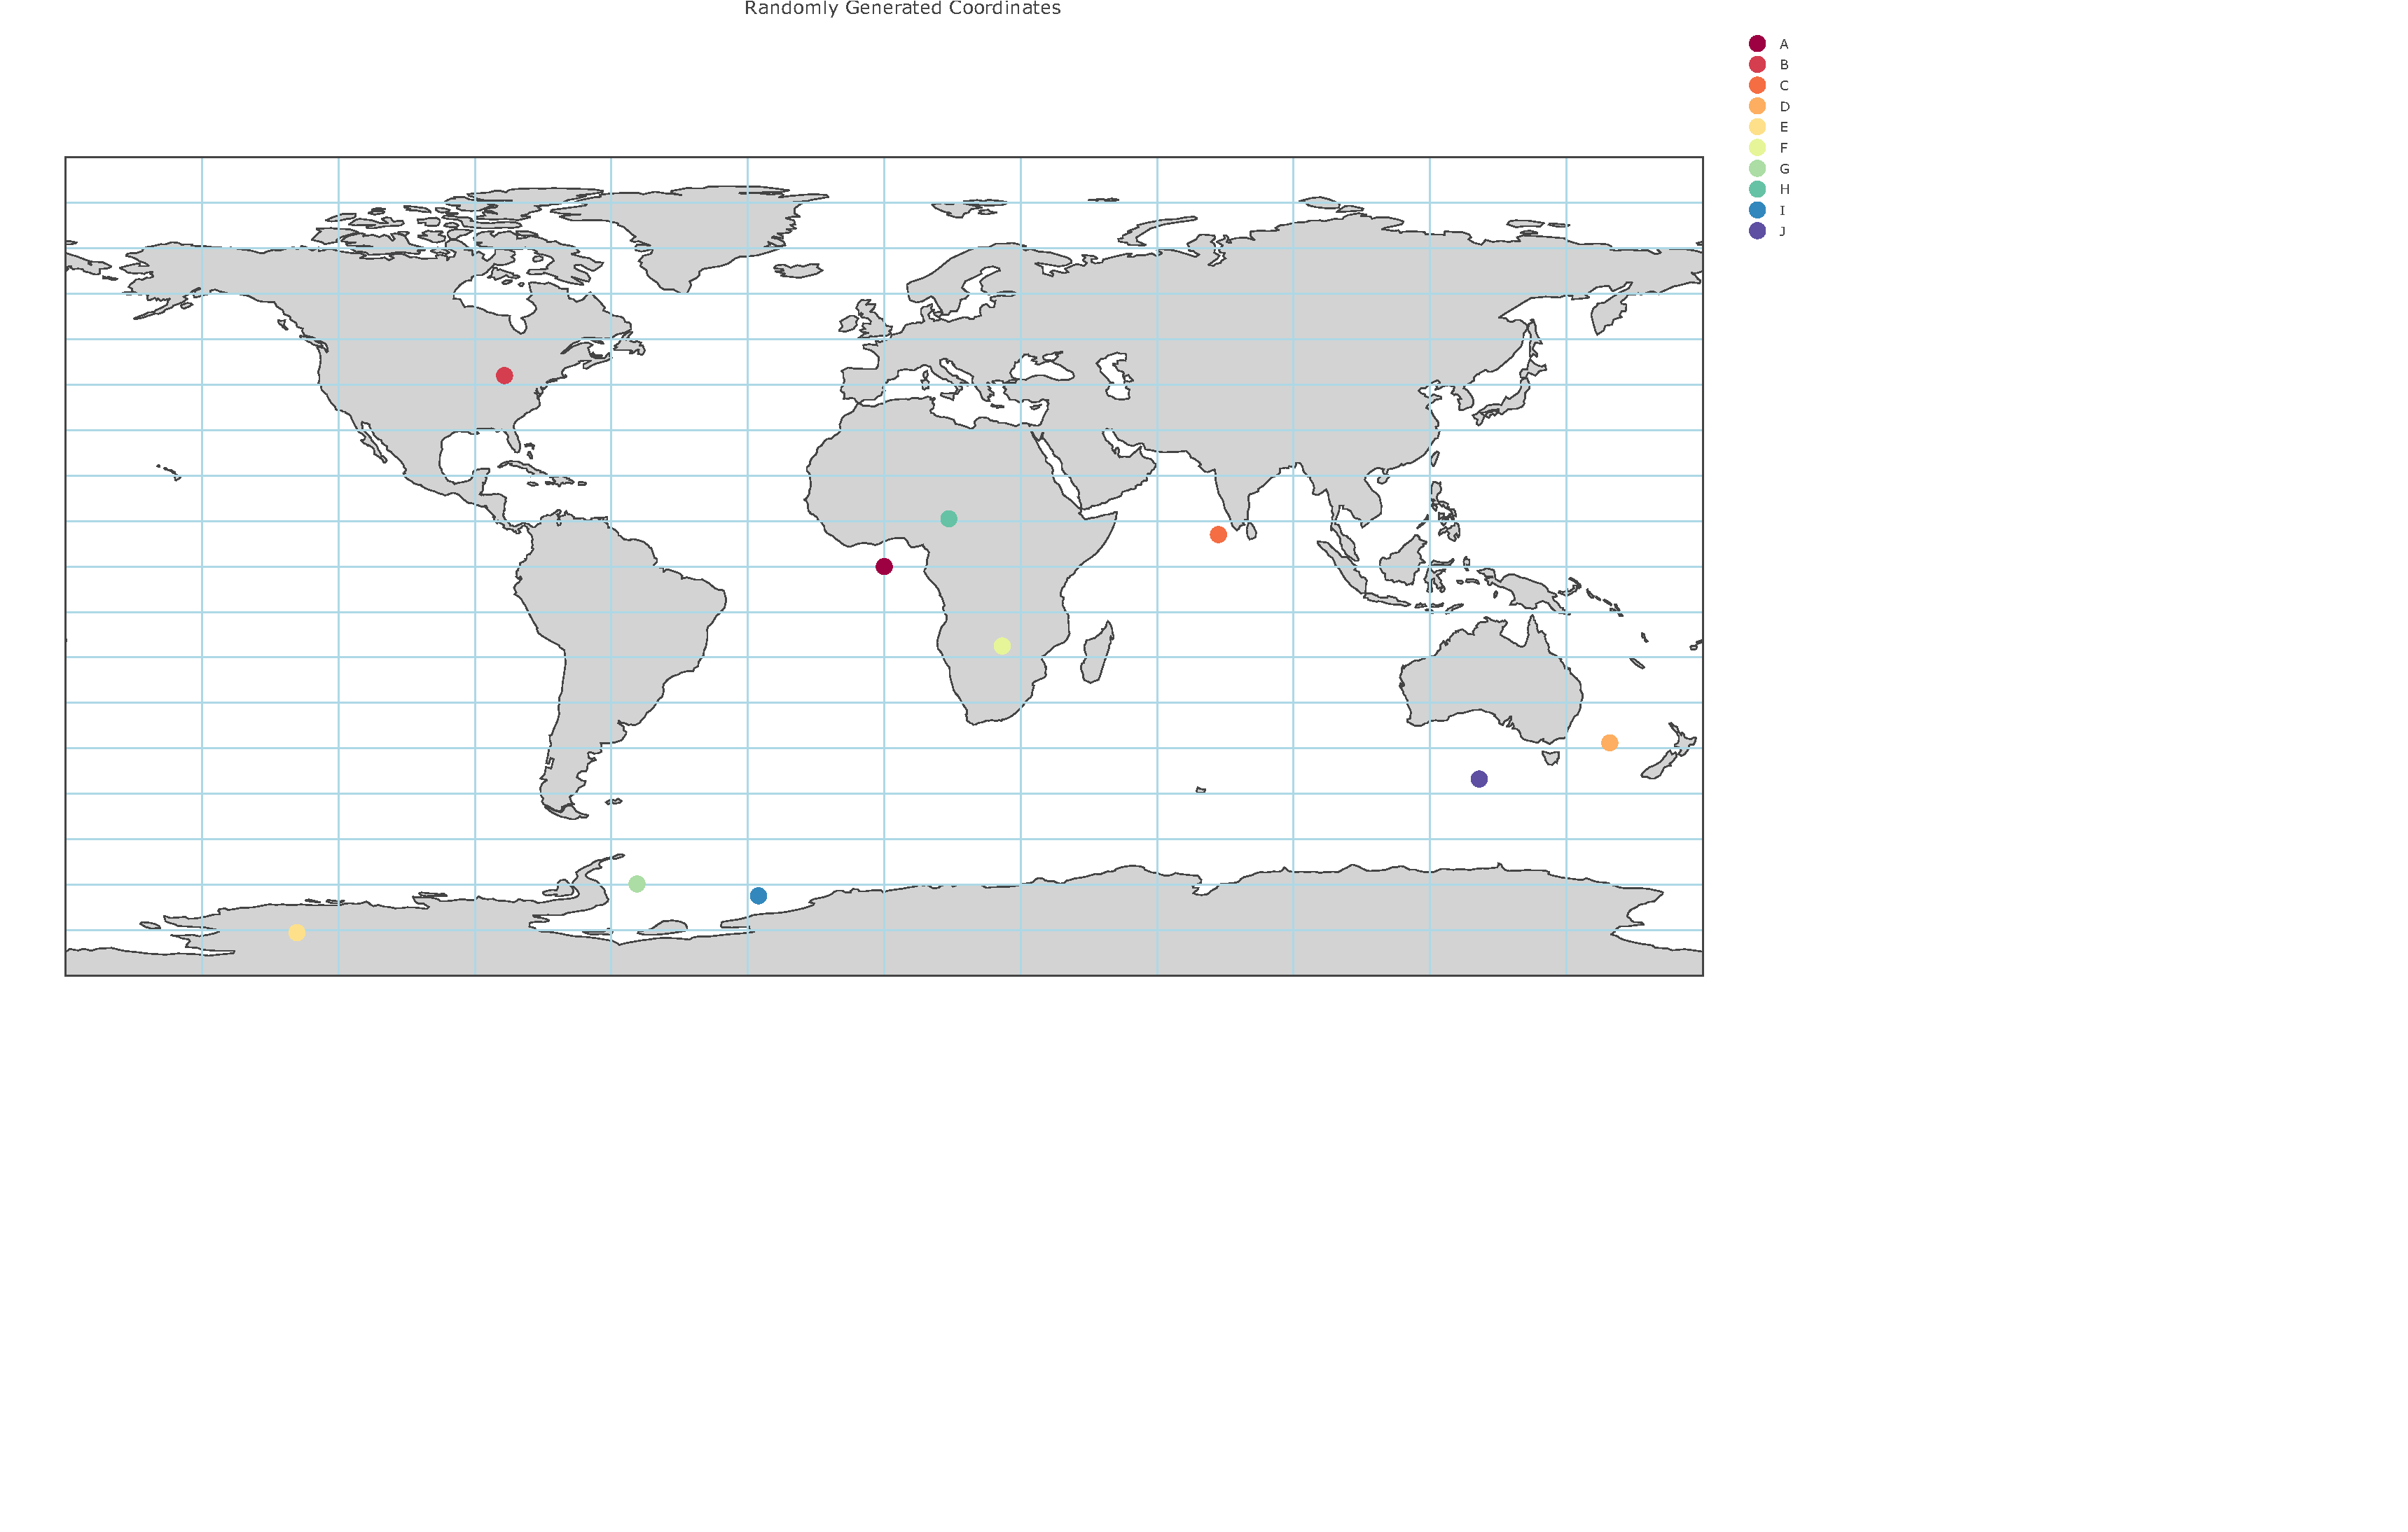
\includegraphics{latitude-and-longitude_files/figure-pdf/unnamed-chunk-3-1.pdf}

\chapter{Map Projections}\label{sec-projections}

Map projections exist because we are trying to take the round globe of
the earth, and project it onto a 2 dimensional surface. Because a
spherical globe can not be projected onto a flat surface without
\emph{some} distortion, different projections make different choices
about the kind of distortion involved.

\begin{figure}[H]

{\centering 
\includegraphics{projections_files/figure-pdf/globe-and-flat-map-1.pdf}

}

\caption{A Globe And A Flat Map}

\end{figure}%

\begin{tcolorbox}[enhanced jigsaw, opacityback=0, colback=white, toprule=.15mm, colframe=quarto-callout-note-color-frame, bottomrule=.15mm, title=\textcolor{quarto-callout-note-color}{\faInfo}\hspace{0.5em}{Note}, coltitle=black, toptitle=1mm, bottomtitle=1mm, arc=.35mm, breakable, colbacktitle=quarto-callout-note-color!10!white, left=2mm, rightrule=.15mm, titlerule=0mm, leftrule=.75mm, opacitybacktitle=0.6]

This chapter is mostly a conceptual overview, and not code-focused.
However, the code is provided for the sake of transparency and teaching.
It is not necessary to understand the code here. But I learned a lot
from: \url{https://plotly.com/r/\#maps}.

\end{tcolorbox}

\section{Set Up The Map}\label{set-up-the-map}

\section{\texorpdfstring{Call \texttt{plotly}
Library}{Call plotly Library}}\label{call-plotly-library}

\begin{Shaded}
\begin{Highlighting}[]
\FunctionTok{library}\NormalTok{(plotly)}
\end{Highlighting}
\end{Shaded}

\section{A Basic Map}\label{a-basic-map}

\begin{Shaded}
\begin{Highlighting}[]
\CommentTok{\# a very basic map could be created with: }

\FunctionTok{library}\NormalTok{(plotly)}

\NormalTok{mymap0 }\OtherTok{\textless{}{-}} \FunctionTok{plot\_geo}\NormalTok{() }\CommentTok{\# create basic map; read into mymap0}

\NormalTok{mymap0 }\CommentTok{\# replay}
\end{Highlighting}
\end{Shaded}


\includegraphics{projections_files/figure-pdf/unnamed-chunk-3-1.pdf}

\section{A More Advanced Map}\label{a-more-advanced-map}

\begin{tcolorbox}[enhanced jigsaw, opacityback=0, colback=white, toprule=.15mm, colframe=quarto-callout-note-color-frame, bottomrule=.15mm, title=\textcolor{quarto-callout-note-color}{\faInfo}\hspace{0.5em}{Note}, coltitle=black, toptitle=1mm, bottomtitle=1mm, arc=.35mm, breakable, colbacktitle=quarto-callout-note-color!10!white, left=2mm, rightrule=.15mm, titlerule=0mm, leftrule=.75mm, opacitybacktitle=0.6]

Again, it is not necessary to understand the code to understand the
conceptual ideas of this chapter. The code below--especially the first
code chunk--is admittedly a little complicated, mostly because I added
options to get the map to look exactly the way that I wanted.

\end{tcolorbox}

\begin{Shaded}
\begin{Highlighting}[]
\NormalTok{mymap }\OtherTok{\textless{}{-}} \FunctionTok{plot\_geo}\NormalTok{() }\SpecialCharTok{\%\textgreater{}\%}
  \FunctionTok{layout}\NormalTok{(}\AttributeTok{title =} \StringTok{"Demonstration Map"}\NormalTok{, }
         \AttributeTok{geo =} \FunctionTok{list}\NormalTok{(}\AttributeTok{showland =} \ConstantTok{TRUE}\NormalTok{, }\CommentTok{\# show land}
                    \AttributeTok{landcolor =} \FunctionTok{toRGB}\NormalTok{(}\StringTok{"darkgrey"}\NormalTok{), }\CommentTok{\# land color}
                    \AttributeTok{showcountries =} \ConstantTok{TRUE}\NormalTok{, }\CommentTok{\# show countries}
                    \AttributeTok{showocean =} \ConstantTok{FALSE}\NormalTok{, }\CommentTok{\# show ocean}
                    \AttributeTok{oceancolor =} \StringTok{"lightblue"}\NormalTok{, }\CommentTok{\# ocean color}
                    \AttributeTok{lataxis =} \FunctionTok{list}\NormalTok{(}\AttributeTok{showgrid =} \ConstantTok{TRUE}\NormalTok{, }\CommentTok{\# latitude options}
                                   \AttributeTok{gridcolor =} \FunctionTok{toRGB}\NormalTok{(}\StringTok{"grey"}\NormalTok{)),}
                    \AttributeTok{lonaxis =} \FunctionTok{list}\NormalTok{(}\AttributeTok{showgrid =} \ConstantTok{TRUE}\NormalTok{, }\CommentTok{\# longitude options}
                                   \AttributeTok{gridcolor =} \FunctionTok{toRGB}\NormalTok{(}\StringTok{"grey"}\NormalTok{)))) }

\NormalTok{mymap }\CommentTok{\# replay}
\end{Highlighting}
\end{Shaded}

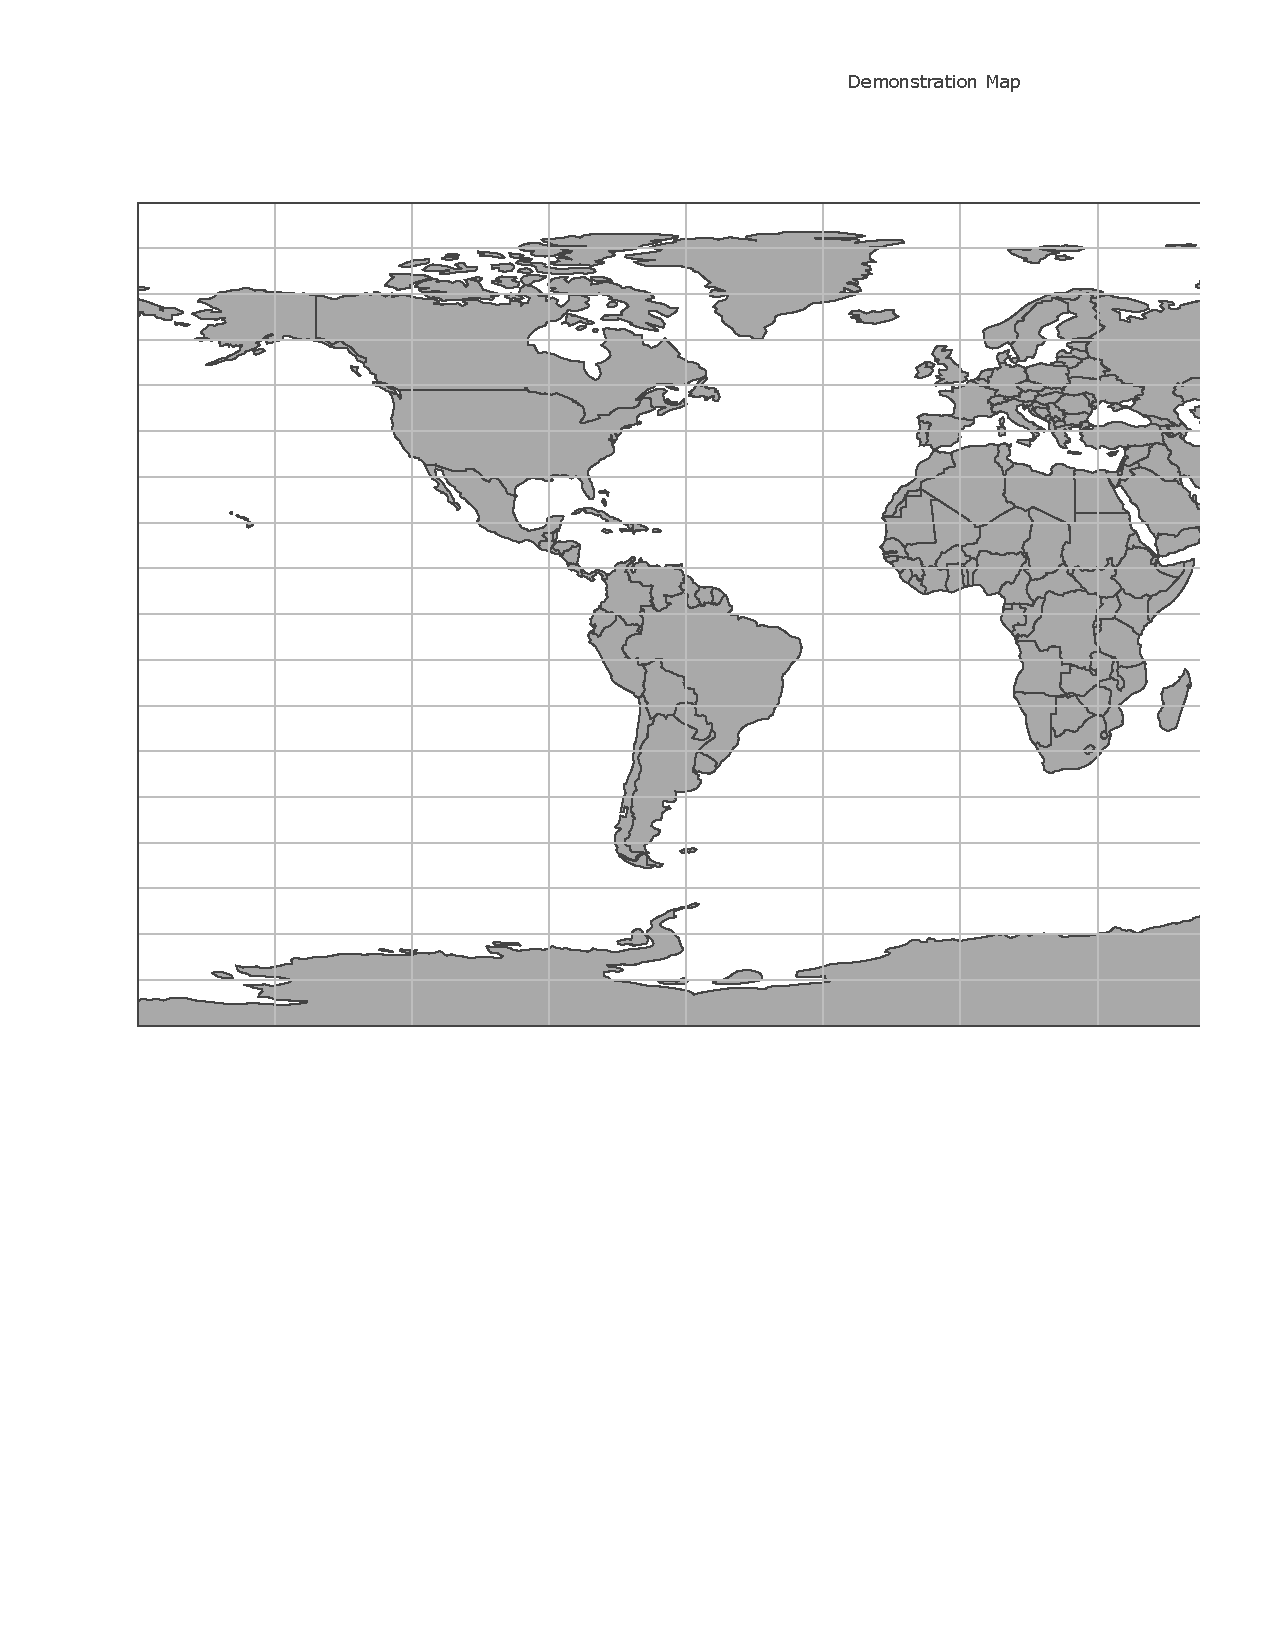
\includegraphics{projections_files/figure-pdf/unnamed-chunk-4-1.pdf}

\section{Map Projections}\label{map-projections}

\subsection{Globe (Orthographic)}\label{globe-orthographic}

\begin{quote}
An \emph{orthographic} projection reprsents the globe with 3 dimensional
accuracy.
\end{quote}

\begin{Shaded}
\begin{Highlighting}[]
\NormalTok{mymap }\SpecialCharTok{\%\textgreater{}\%} 
  \FunctionTok{layout}\NormalTok{(}\AttributeTok{geo =} \FunctionTok{list}\NormalTok{(}\AttributeTok{projection =} \FunctionTok{list}\NormalTok{(}\AttributeTok{type =} \StringTok{\textquotesingle{}orthographic\textquotesingle{}}\NormalTok{)))}
\end{Highlighting}
\end{Shaded}

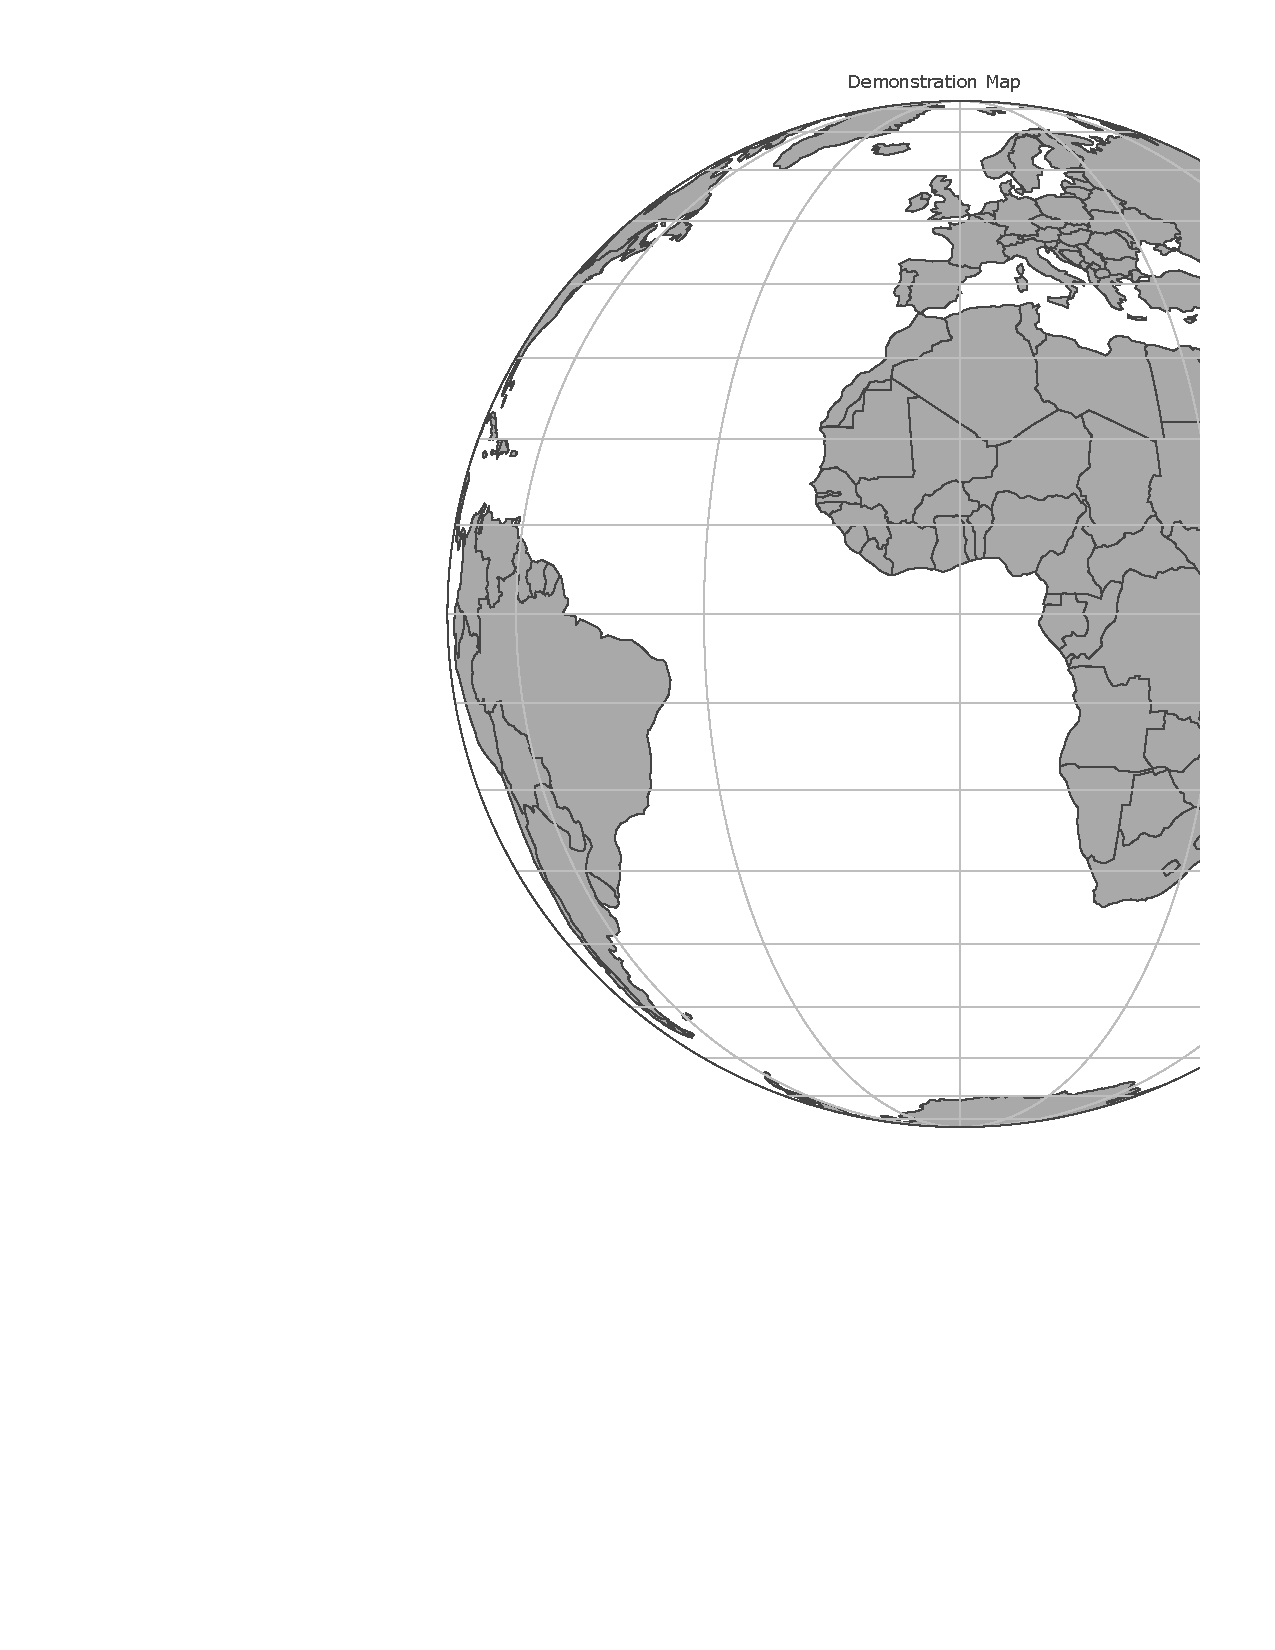
\includegraphics{projections_files/figure-pdf/unnamed-chunk-5-1.pdf}

\subsection{Mercator}\label{mercator}

\begin{quote}
A \emph{Mercator} projection reprsents the earth with perpendicular
latitude and longitude. This projection can be helpful in some kinds of
navigation, but areas of landmasses are distorted, especially as one
approaches the poles.
\end{quote}

\begin{Shaded}
\begin{Highlighting}[]
\NormalTok{mymap }\SpecialCharTok{\%\textgreater{}\%} 
  \FunctionTok{layout}\NormalTok{(}\AttributeTok{geo=}\FunctionTok{list}\NormalTok{(}\AttributeTok{projection =} \FunctionTok{list}\NormalTok{(}\AttributeTok{type =} \StringTok{\textquotesingle{}mercator\textquotesingle{}}\NormalTok{)))}
\end{Highlighting}
\end{Shaded}

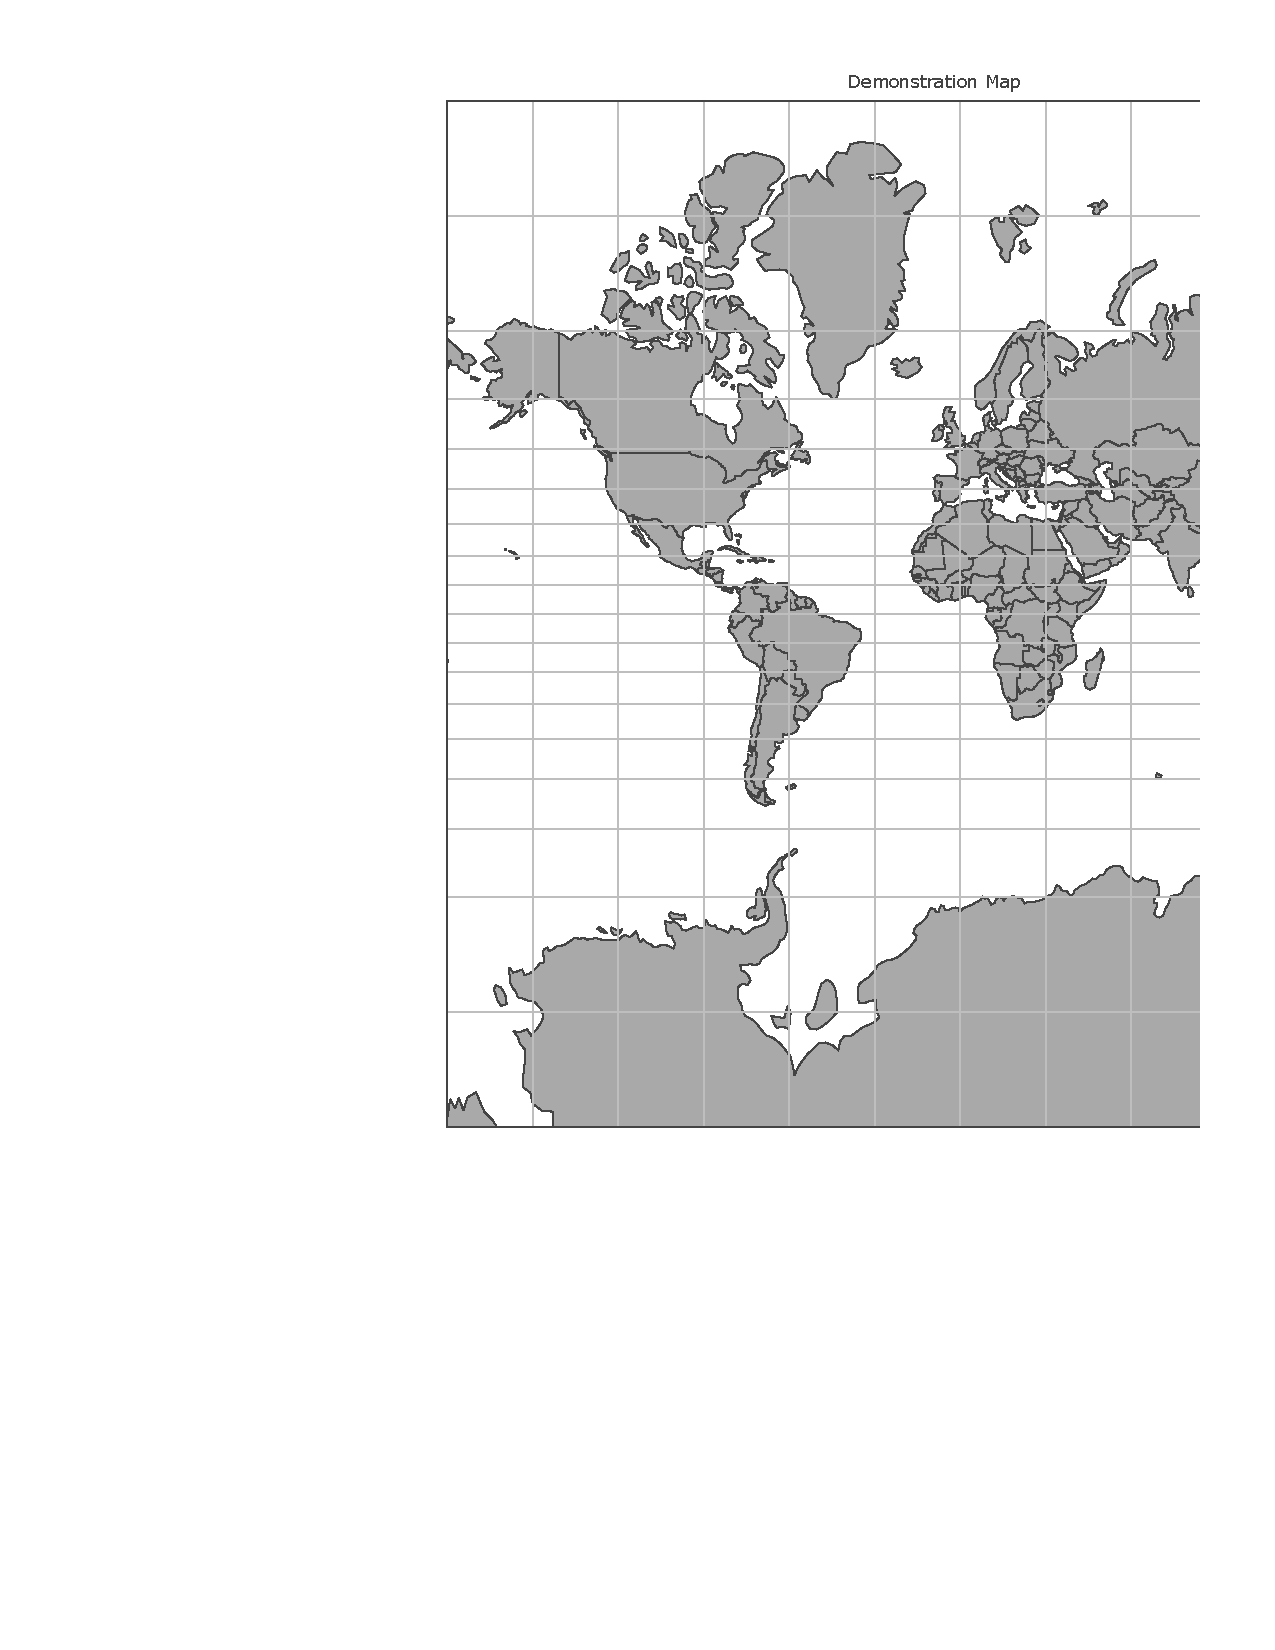
\includegraphics{projections_files/figure-pdf/unnamed-chunk-6-1.pdf}

\subsection{Mollweide}\label{mollweide}

\begin{quote}
The \emph{Mollweide} projection is an \emph{equal area} projection. As a
consequence, latitude and longitude lines are not perpendicular, and the
shapes of some landmasses may appear to be distorted.
\end{quote}

\begin{Shaded}
\begin{Highlighting}[]
\NormalTok{mymap }\SpecialCharTok{\%\textgreater{}\%} 
  \FunctionTok{layout}\NormalTok{(}\AttributeTok{geo=}\FunctionTok{list}\NormalTok{(}\AttributeTok{projection =} \FunctionTok{list}\NormalTok{(}\AttributeTok{type =} \StringTok{\textquotesingle{}mollweide\textquotesingle{}}\NormalTok{)))}
\end{Highlighting}
\end{Shaded}

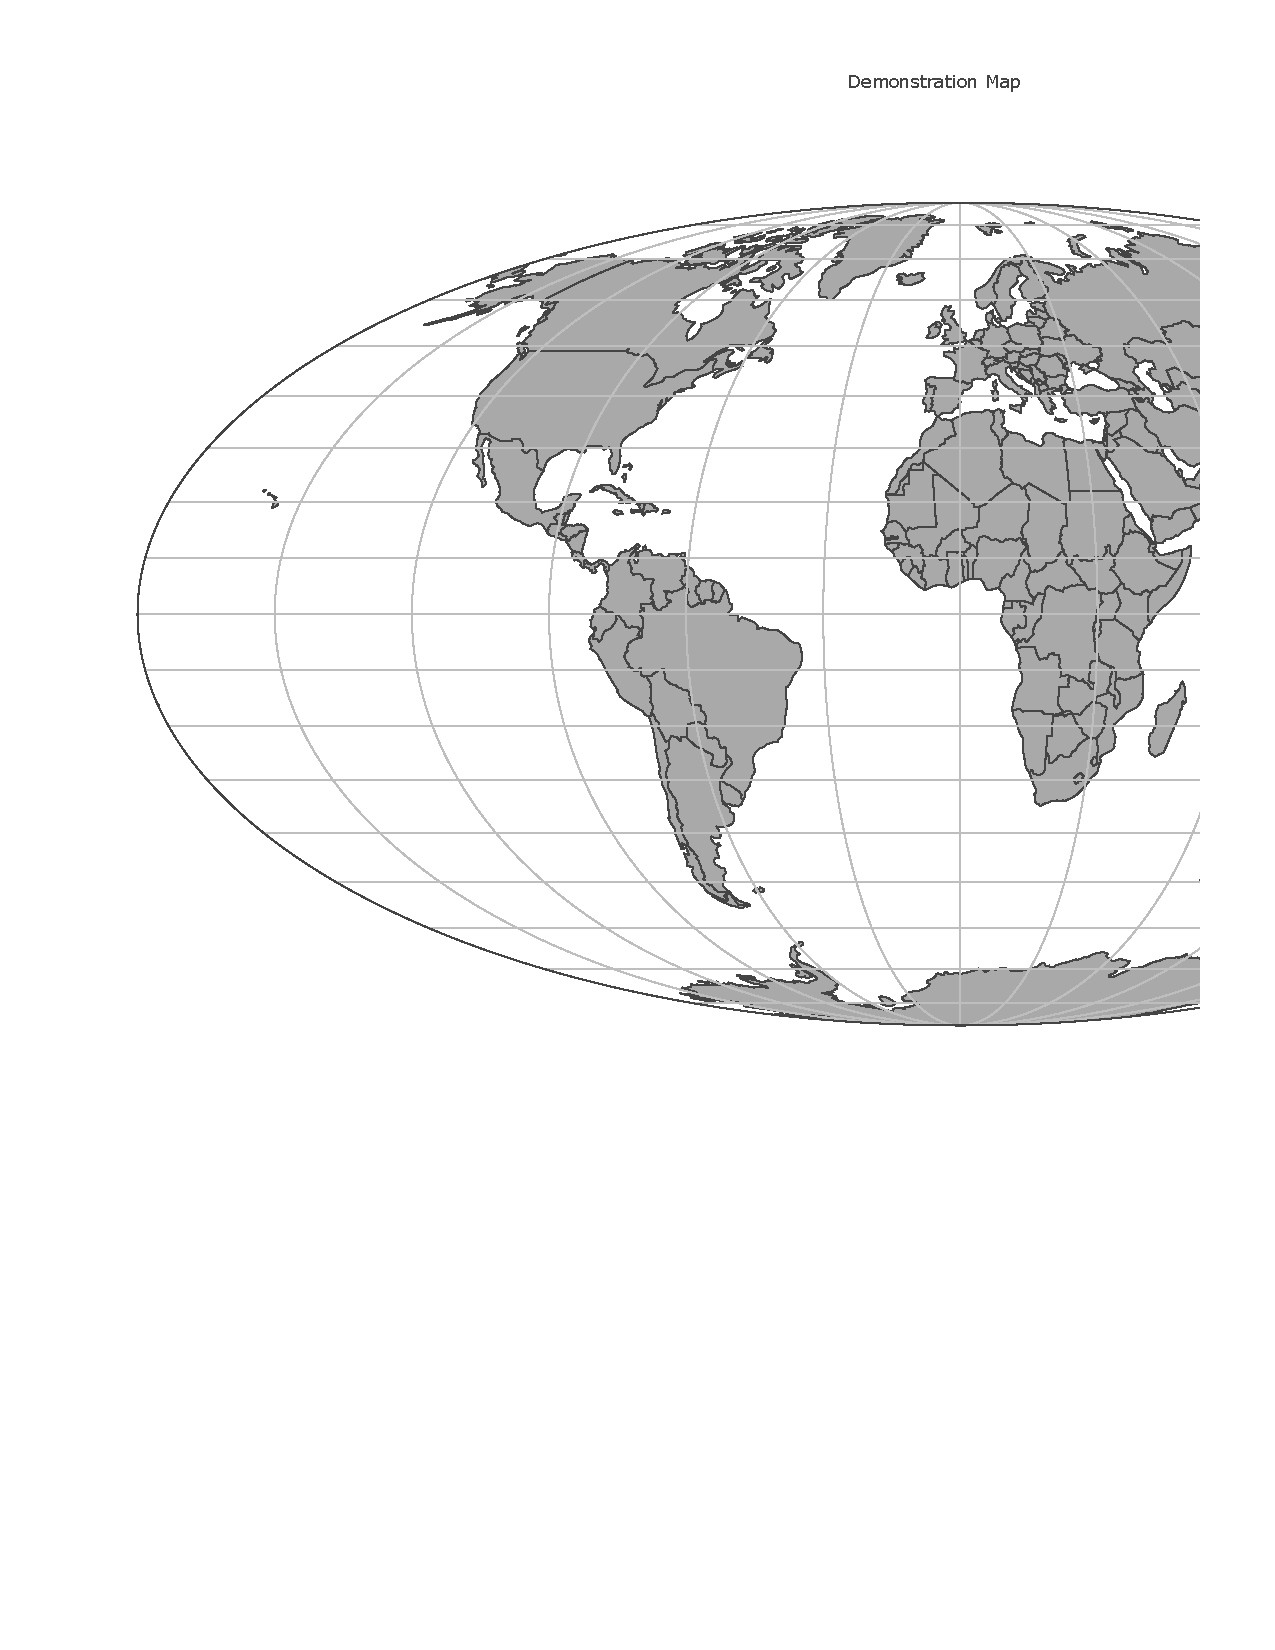
\includegraphics{projections_files/figure-pdf/unnamed-chunk-7-1.pdf}

\subsection{Robinson}\label{robinson}

\begin{quote}
The \emph{Robinson} projection is an attempt to compromise between equal
areas and a natural looking map.
\end{quote}

\begin{Shaded}
\begin{Highlighting}[]
\NormalTok{mymap }\SpecialCharTok{\%\textgreater{}\%} 
  \FunctionTok{layout}\NormalTok{(}\AttributeTok{geo=}\FunctionTok{list}\NormalTok{(}\AttributeTok{projection =} \FunctionTok{list}\NormalTok{(}\AttributeTok{type =} \StringTok{\textquotesingle{}robinson\textquotesingle{}}\NormalTok{)))}
\end{Highlighting}
\end{Shaded}

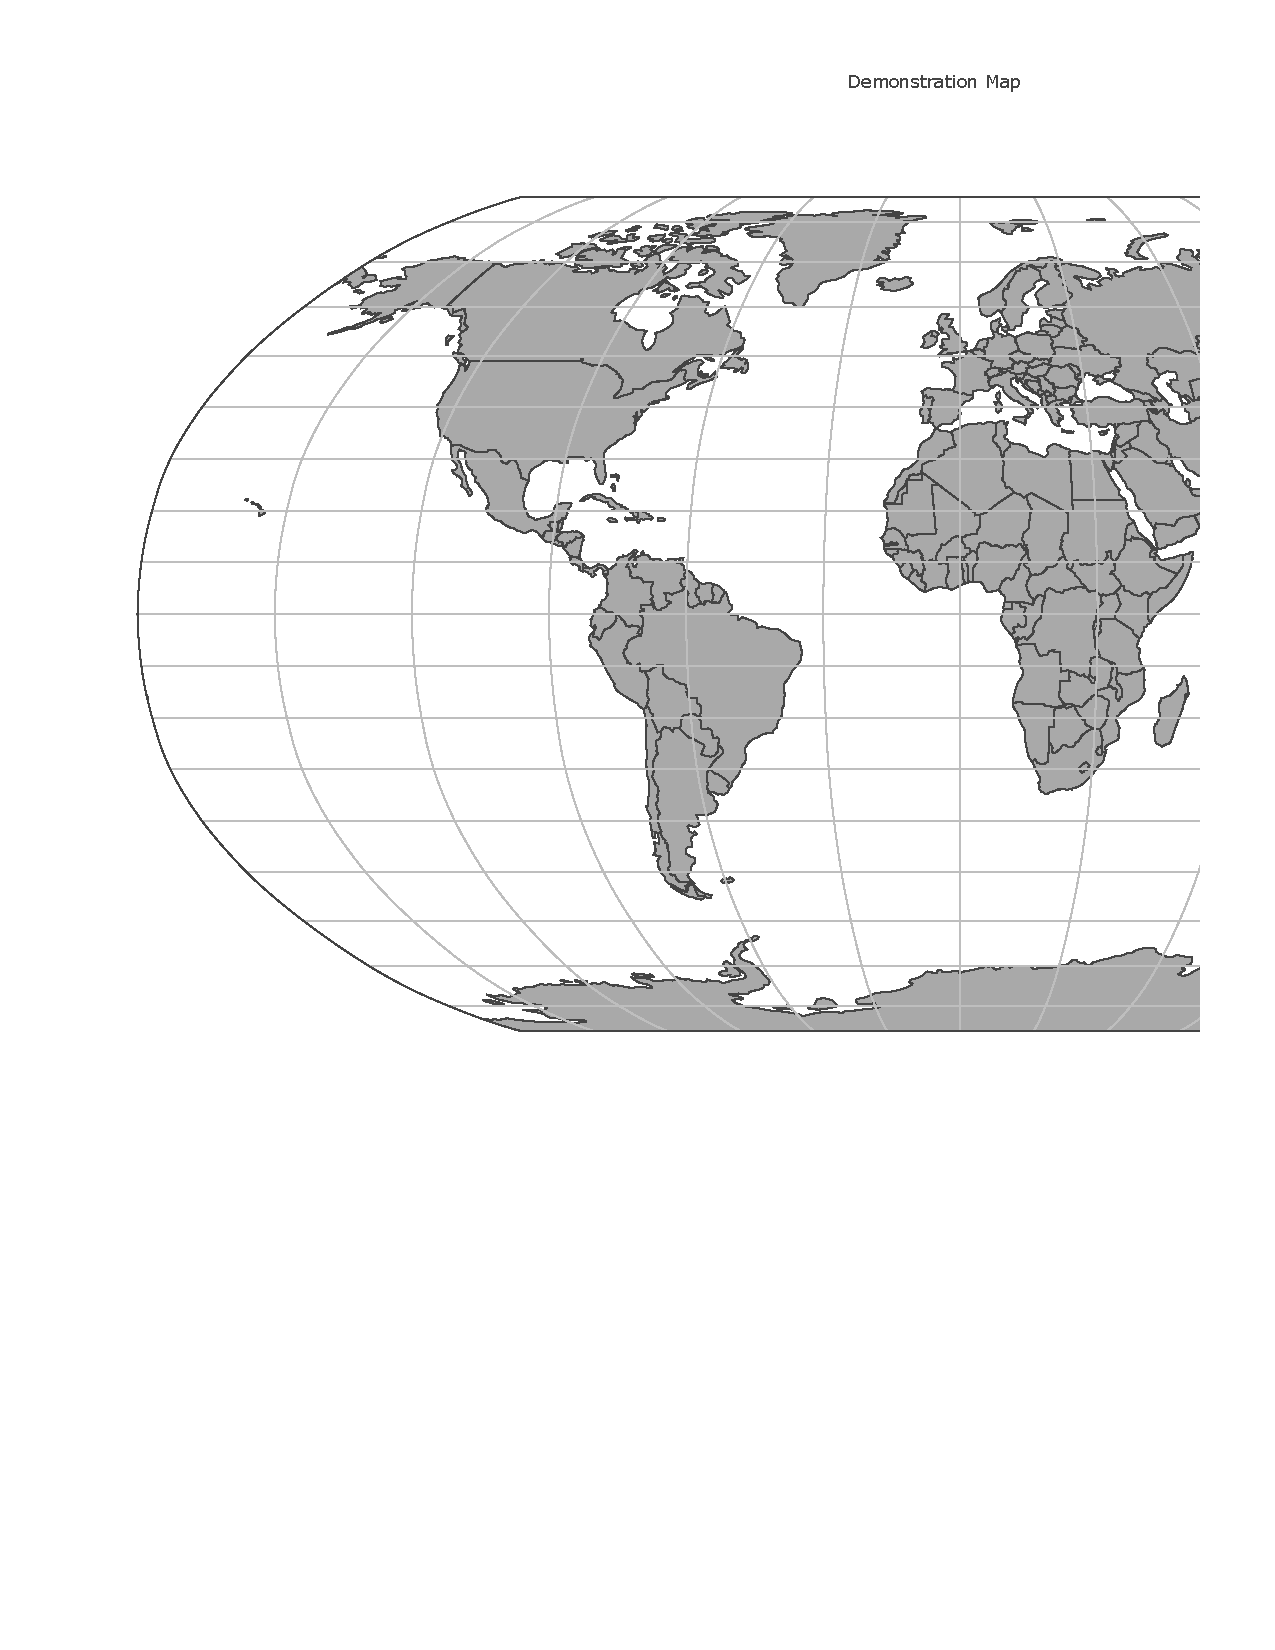
\includegraphics{projections_files/figure-pdf/unnamed-chunk-8-1.pdf}

\chapter{Coordinate Reference Systems
(CRS)}\label{coordinate-reference-systems-crs}

\section{Coordinate Reference
Systems}\label{coordinate-reference-systems}

\begin{quote}
``Map projections try to portray the surface of the earth or a portion
of the earth on a flat piece of paper or computer screen. A coordinate
reference system (CRS) then defines, with the help of coordinates, how
the two-dimensional, projected map in your GIS is related to real places
on the earth. The decision as to which map projection and coordinate
reference system to use, depends on the regional extent of the area you
want to work in, on the analysis you want to do and often on the
availability of data.'' From
\href{https://docs.qgis.org/2.8/en/docs/gentle_gis_introduction/coordinate_reference_systems.html}{qgis.org}
\end{quote}

\section{Call Libraries}\label{call-libraries}

\begin{Shaded}
\begin{Highlighting}[]
\FunctionTok{library}\NormalTok{(sf) }\CommentTok{\# simple (spatial) features}

\FunctionTok{library}\NormalTok{(ggplot2) }\CommentTok{\# beautiful graphs}
\end{Highlighting}
\end{Shaded}

\section{\texorpdfstring{Open \texttt{wrld\_simpl}
Shapefile}{Open wrld\_simpl Shapefile}}\label{open-wrld_simpl-shapefile}

\begin{Shaded}
\begin{Highlighting}[]
\NormalTok{world }\OtherTok{\textless{}{-}} \FunctionTok{read\_sf}\NormalTok{(}\StringTok{"./shapefiles/wrld\_simpl/wrld\_simpl.shp"}\NormalTok{)}
\end{Highlighting}
\end{Shaded}

\begin{Shaded}
\begin{Highlighting}[]
\FunctionTok{head}\NormalTok{(world) }\CommentTok{\# show the top (head) of the data}
\end{Highlighting}
\end{Shaded}

\begin{verbatim}
Simple feature collection with 6 features and 10 fields
Geometry type: MULTIPOLYGON
Dimension:     XY
Bounding box:  xmin: -61.88722 ymin: -18.01639 xmax: 50.37499 ymax: 42.61805
Geodetic CRS:  +proj=longlat +datum=WGS84 +no_defs
# A tibble: 6 x 11
  FIPS  ISO2  ISO3     UN NAME                AREA REGION SUBREGION    LON   LAT
  <chr> <chr> <chr> <int> <chr>              <int>  <int>     <int>  <dbl> <dbl>
1 AC    AG    ATG      28 Antigua and Barb~     44     19        29 -61.8   17.1
2 AG    DZ    DZA      12 Algeria           238174      2        15   2.63  28.2
3 AJ    AZ    AZE      31 Azerbaijan          8260    142       145  47.4   40.4
4 AL    AL    ALB       8 Albania             2740    150        39  20.1   41.1
5 AM    AM    ARM      51 Armenia             2820    142       145  44.6   40.5
6 AO    AO    AGO      24 Angola            124670      2        17  17.5  -12.3
# i 1 more variable: geometry <MULTIPOLYGON [°]>
\end{verbatim}

\section{\texorpdfstring{Find Out the CRS of
\texttt{wrld\_simpl}}{Find Out the CRS of wrld\_simpl}}\label{find-out-the-crs-of-wrld_simpl}

As with many global data sets (and many other data sets),
\texttt{wrld\_simpl} uses \emph{World Geodetic System 1984}.

\begin{Shaded}
\begin{Highlighting}[]
\FunctionTok{st\_crs}\NormalTok{(world)}
\end{Highlighting}
\end{Shaded}

\begin{verbatim}
Coordinate Reference System:
  User input: unknown 
  wkt:
GEOGCRS["unknown",
    DATUM["World Geodetic System 1984",
        ELLIPSOID["WGS 84",6378137,298.257223563,
            LENGTHUNIT["metre",1]],
        ID["EPSG",6326]],
    PRIMEM["Greenwich",0,
        ANGLEUNIT["Degree",0.0174532925199433]],
    CS[ellipsoidal,2],
        AXIS["longitude",east,
            ORDER[1],
            ANGLEUNIT["Degree",0.0174532925199433]],
        AXIS["latitude",north,
            ORDER[2],
            ANGLEUNIT["Degree",0.0174532925199433]]]
\end{verbatim}

\section{\texorpdfstring{Plot The \texttt{wrld\_simpl}
Data}{Plot The wrld\_simpl Data}}\label{plot-the-wrld_simpl-data}

\begin{Shaded}
\begin{Highlighting}[]
\FunctionTok{ggplot}\NormalTok{(world) }\SpecialCharTok{+} 
  \FunctionTok{geom\_sf}\NormalTok{() }\SpecialCharTok{+}
  \FunctionTok{theme\_minimal}\NormalTok{()}
\end{Highlighting}
\end{Shaded}

\includegraphics{crs_files/figure-pdf/unnamed-chunk-5-1.pdf}

\part{GIS Data}

\chapter{\texorpdfstring{Simple Features
(\texttt{sf})}{Simple Features (sf)}}\label{sec-sf}

R's new preferred way of handling spatial data seems to be \emph{simple
features} (\texttt{sf}).

Use \texttt{library(sf)} to read, write and manipulate \emph{simple
features}.

Other forms of data such as \emph{shapefiles}
(Chapter~\ref{sec-shapefiles}) often need to be read as simple features.

Mapping routines such as \texttt{ggplot} (Chapter~\ref{sec-ggplot-map})
will also often want data to be in the form of \emph{simple features}.

\chapter{Shapefiles}\label{sec-shapefiles}

\section{Introduction}\label{introduction-2}

Shapefiles are a spatial data format originally developed by
\href{https://www.esri.com/en-us/home}{ESRI}.

Shapefiles come in three major types:

\begin{itemize}
\tightlist
\item
  \textbf{points} {●}, to represent point features such as individual or
  agency locations. At larger scales, cities or towns might also be
  points.
\item
  \textbf{lines}️ {━━━}, to represent line features such as roads,
  trails, or rivers.
\item
  \textbf{polygons} {▭▯}, to represent polygon features such as outlines
  of cities, states, or countries.
\end{itemize}

\section{\texorpdfstring{Shape\emph{files} Are Actually
\emph{Collections} of
Files}{Shapefiles Are Actually Collections of Files}}\label{shapefiles-are-actually-collections-of-files}

Shape\emph{files} are actually a \emph{set} or \emph{collection} of
associated files, all with the same name, and all in the same directory,
but different suffixes.

R--and many other software programs--generally reference the
\texttt{*.shp} file of the shapefile.

\begin{Shaded}
\begin{Highlighting}[]
\FunctionTok{list.files}\NormalTok{(}\StringTok{"./shapefiles/a2trees"}\NormalTok{)}
\end{Highlighting}
\end{Shaded}

\begin{verbatim}
[1] "AA_Trees.cpg"     "AA_Trees.dbf"     "AA_Trees.prj"     "AA_Trees.sbn"    
[5] "AA_Trees.sbx"     "AA_Trees.shp"     "AA_Trees.shp.xml" "AA_Trees.shx"    
\end{verbatim}

\section{Call Libraries}\label{call-libraries-1}

\begin{Shaded}
\begin{Highlighting}[]
\FunctionTok{library}\NormalTok{(ggplot2) }\CommentTok{\# beautiful graphs}

\FunctionTok{library}\NormalTok{(sf) }\CommentTok{\# simple (spatial) features}
\end{Highlighting}
\end{Shaded}

\section{Open Shapefiles}\label{open-shapefiles}

\begin{Shaded}
\begin{Highlighting}[]
\NormalTok{city\_boundary }\OtherTok{\textless{}{-}} \FunctionTok{read\_sf}\NormalTok{(}\StringTok{"./shapefiles/AA\_City\_Boundary/AA\_City\_Boundary.shp"}\NormalTok{)}

\NormalTok{buildings }\OtherTok{\textless{}{-}} \FunctionTok{read\_sf}\NormalTok{(}\StringTok{"./shapefiles/AA\_Building\_Footprints/AA\_Building\_Footprints.shp"}\NormalTok{)}

\CommentTok{\# trees \textless{}{-} read\_sf("./shapefiles/a2trees/AA\_Trees.shp")}

\CommentTok{\# parks \textless{}{-} read\_sf("./shapefiles/AA\_Parks/AA\_Parks.shp")}

\CommentTok{\# university \textless{}{-} read\_sf("./shapefiles/AA\_University/AA\_University.shp")}

\NormalTok{clients }\OtherTok{\textless{}{-}} \FunctionTok{read\_sf}\NormalTok{(}\StringTok{"./shapefiles/clients/clients.shp"}\NormalTok{)}

\NormalTok{WashtenawRoads }\OtherTok{\textless{}{-}} \FunctionTok{read\_sf}\NormalTok{(}\StringTok{"./shapefiles/Roads/RoadCenterlines.shp"}\NormalTok{)}

\NormalTok{AnnArborRoads }\OtherTok{\textless{}{-}} \FunctionTok{st\_crop}\NormalTok{(WashtenawRoads, }
\NormalTok{                         city\_boundary) }\CommentTok{\# crop to only get A2 roads}

\CommentTok{\# watersheds \textless{}{-} read\_sf("./shapefiles/watersheds/Watersheds.shp")}
\end{Highlighting}
\end{Shaded}

\section{\texorpdfstring{Use \texttt{ggplot} to Map the
Shapefiles}{Use ggplot to Map the Shapefiles}}\label{use-ggplot-to-map-the-shapefiles}

\begin{Shaded}
\begin{Highlighting}[]
\FunctionTok{ggplot}\NormalTok{(city\_boundary) }\SpecialCharTok{+} \CommentTok{\# initial sf data}
  \CommentTok{\# geom\_sf(data = buildings,}
  \CommentTok{\#         fill = "lightgrey") +}
  \FunctionTok{geom\_sf}\NormalTok{(}\AttributeTok{data =}\NormalTok{ AnnArborRoads, }\CommentTok{\# first layer: Ann Arbor roads }
          \AttributeTok{color =} \StringTok{"lightgrey"}\NormalTok{) }\SpecialCharTok{+}
  \FunctionTok{geom\_sf}\NormalTok{(}\AttributeTok{color =} \StringTok{"red"}\NormalTok{, }\CommentTok{\# second layer: city boundary}
          \AttributeTok{alpha =}\NormalTok{ .}\DecValTok{5}\NormalTok{) }\SpecialCharTok{+} 
  \FunctionTok{geom\_sf}\NormalTok{(}\AttributeTok{data =}\NormalTok{ clients, }\CommentTok{\# third layer: clients}
          \AttributeTok{size =} \DecValTok{1}\NormalTok{,}
          \AttributeTok{color =} \StringTok{"purple"}\NormalTok{) }\SpecialCharTok{+}
  \FunctionTok{labs}\NormalTok{(}\AttributeTok{title =} \StringTok{"Demonstration of Shapefiles"}\NormalTok{,}
       \AttributeTok{subtitle =} \StringTok{"Purple Clients Are Points }\SpecialCharTok{\textbackslash{}n}\StringTok{Grey Roads are Lines }\SpecialCharTok{\textbackslash{}n}\StringTok{Red City Boundary is Polygon"}\NormalTok{) }\SpecialCharTok{+}
  \FunctionTok{theme\_minimal}\NormalTok{() }\SpecialCharTok{+}
  \FunctionTok{theme}\NormalTok{(}\AttributeTok{axis.text =} \FunctionTok{element\_text}\NormalTok{(}\AttributeTok{size =} \FunctionTok{rel}\NormalTok{(.}\DecValTok{5}\NormalTok{)))}
\end{Highlighting}
\end{Shaded}

\includegraphics{shapefiles_files/figure-pdf/unnamed-chunk-4-1.pdf}

\chapter{Shapefiles on This Site}\label{sec-shapefiles2}

For user convenience, these shapefiles are available on this site.

\includegraphics{shapefiles2_files/figure-pdf/unnamed-chunk-1-1.pdf}

\chapter{Inspecting Geographic Data Files}\label{sec-inspecting}

Often, when we open a new geographic data file, we don't know what
fields of data it contains.

It is useful to get an idea of what data our geographic data file
already contains in order to know whether or not we may need to merge in
other data (Chapter~\ref{sec-merging}).

\texttt{names} and \texttt{head} are two useful commands for learning
about new geographic data files.

As an example, I am going to use the country data from the
\texttt{rnaturalearth} library (Chapter~\ref{sec-rnaturalearth}).

\section{Data}\label{data}

I use \texttt{ne\_countries()} to create the \texttt{mapdata} dataset as
an \texttt{sf} object (Chapter~\ref{sec-sf}).

\begin{Shaded}
\begin{Highlighting}[]
\FunctionTok{library}\NormalTok{(rnaturalearth) }

\NormalTok{mapdata }\OtherTok{\textless{}{-}} \FunctionTok{ne\_countries}\NormalTok{(}\AttributeTok{scale =} \StringTok{"medium"}\NormalTok{, }
                        \AttributeTok{returnclass =} \StringTok{"sf"}\NormalTok{) }
\end{Highlighting}
\end{Shaded}

\section{names}\label{names}

\texttt{names} gives us the names of all of the fields of the data.

\begin{Shaded}
\begin{Highlighting}[]
\FunctionTok{names}\NormalTok{(mapdata)}
\end{Highlighting}
\end{Shaded}

\begin{verbatim}
  [1] "featurecla" "scalerank"  "labelrank"  "sovereignt" "sov_a3"    
  [6] "adm0_dif"   "level"      "type"       "tlc"        "admin"     
 [11] "adm0_a3"    "geou_dif"   "geounit"    "gu_a3"      "su_dif"    
 [16] "subunit"    "su_a3"      "brk_diff"   "name"       "name_long" 
 [21] "brk_a3"     "brk_name"   "brk_group"  "abbrev"     "postal"    
 [26] "formal_en"  "formal_fr"  "name_ciawf" "note_adm0"  "note_brk"  
 [31] "name_sort"  "name_alt"   "mapcolor7"  "mapcolor8"  "mapcolor9" 
 [36] "mapcolor13" "pop_est"    "pop_rank"   "pop_year"   "gdp_md"    
 [41] "gdp_year"   "economy"    "income_grp" "fips_10"    "iso_a2"    
 [46] "iso_a2_eh"  "iso_a3"     "iso_a3_eh"  "iso_n3"     "iso_n3_eh" 
 [51] "un_a3"      "wb_a2"      "wb_a3"      "woe_id"     "woe_id_eh" 
 [56] "woe_note"   "adm0_iso"   "adm0_diff"  "adm0_tlc"   "adm0_a3_us"
 [61] "adm0_a3_fr" "adm0_a3_ru" "adm0_a3_es" "adm0_a3_cn" "adm0_a3_tw"
 [66] "adm0_a3_in" "adm0_a3_np" "adm0_a3_pk" "adm0_a3_de" "adm0_a3_gb"
 [71] "adm0_a3_br" "adm0_a3_il" "adm0_a3_ps" "adm0_a3_sa" "adm0_a3_eg"
 [76] "adm0_a3_ma" "adm0_a3_pt" "adm0_a3_ar" "adm0_a3_jp" "adm0_a3_ko"
 [81] "adm0_a3_vn" "adm0_a3_tr" "adm0_a3_id" "adm0_a3_pl" "adm0_a3_gr"
 [86] "adm0_a3_it" "adm0_a3_nl" "adm0_a3_se" "adm0_a3_bd" "adm0_a3_ua"
 [91] "adm0_a3_un" "adm0_a3_wb" "continent"  "region_un"  "subregion" 
 [96] "region_wb"  "name_len"   "long_len"   "abbrev_len" "tiny"      
[101] "homepart"   "min_zoom"   "min_label"  "max_label"  "label_x"   
[106] "label_y"    "ne_id"      "wikidataid" "name_ar"    "name_bn"   
[111] "name_de"    "name_en"    "name_es"    "name_fa"    "name_fr"   
[116] "name_el"    "name_he"    "name_hi"    "name_hu"    "name_id"   
[121] "name_it"    "name_ja"    "name_ko"    "name_nl"    "name_pl"   
[126] "name_pt"    "name_ru"    "name_sv"    "name_tr"    "name_uk"   
[131] "name_ur"    "name_vi"    "name_zh"    "name_zht"   "fclass_iso"
[136] "tlc_diff"   "fclass_tlc" "fclass_us"  "fclass_fr"  "fclass_ru" 
[141] "fclass_es"  "fclass_cn"  "fclass_tw"  "fclass_in"  "fclass_np" 
[146] "fclass_pk"  "fclass_de"  "fclass_gb"  "fclass_br"  "fclass_il" 
[151] "fclass_ps"  "fclass_sa"  "fclass_eg"  "fclass_ma"  "fclass_pt" 
[156] "fclass_ar"  "fclass_jp"  "fclass_ko"  "fclass_vn"  "fclass_tr" 
[161] "fclass_id"  "fclass_pl"  "fclass_gr"  "fclass_it"  "fclass_nl" 
[166] "fclass_se"  "fclass_bd"  "fclass_ua"  "geometry"  
\end{verbatim}

\section{head}\label{head}

\texttt{head} shows us the first several rows of data.

\begin{Shaded}
\begin{Highlighting}[]
\FunctionTok{head}\NormalTok{(mapdata)}
\end{Highlighting}
\end{Shaded}

\begin{verbatim}
Simple feature collection with 6 features and 168 fields
Geometry type: MULTIPOLYGON
Dimension:     XY
Bounding box:  xmin: -73.36621 ymin: -22.40205 xmax: 109.4449 ymax: 41.9062
Geodetic CRS:  WGS 84
       featurecla scalerank labelrank sovereignt sov_a3 adm0_dif level
1 Admin-0 country         1         3   Zimbabwe    ZWE        0     2
2 Admin-0 country         1         3     Zambia    ZMB        0     2
3 Admin-0 country         1         3      Yemen    YEM        0     2
4 Admin-0 country         3         2    Vietnam    VNM        0     2
5 Admin-0 country         5         3  Venezuela    VEN        0     2
6 Admin-0 country         6         6    Vatican    VAT        0     2
               type tlc     admin adm0_a3 geou_dif   geounit gu_a3 su_dif
1 Sovereign country   1  Zimbabwe     ZWE        0  Zimbabwe   ZWE      0
2 Sovereign country   1    Zambia     ZMB        0    Zambia   ZMB      0
3 Sovereign country   1     Yemen     YEM        0     Yemen   YEM      0
4 Sovereign country   1   Vietnam     VNM        0   Vietnam   VNM      0
5 Sovereign country   1 Venezuela     VEN        0 Venezuela   VEN      0
6 Sovereign country   1   Vatican     VAT        0   Vatican   VAT      0
    subunit su_a3 brk_diff      name name_long brk_a3  brk_name brk_group
1  Zimbabwe   ZWE        0  Zimbabwe  Zimbabwe    ZWE  Zimbabwe      <NA>
2    Zambia   ZMB        0    Zambia    Zambia    ZMB    Zambia      <NA>
3     Yemen   YEM        0     Yemen     Yemen    YEM     Yemen      <NA>
4   Vietnam   VNM        0   Vietnam   Vietnam    VNM   Vietnam      <NA>
5 Venezuela   VEN        0 Venezuela Venezuela    VEN Venezuela      <NA>
6   Vatican   VAT        0   Vatican   Vatican    VAT   Vatican      <NA>
  abbrev postal                        formal_en
1  Zimb.     ZW             Republic of Zimbabwe
2 Zambia     ZM               Republic of Zambia
3   Yem.     YE                Republic of Yemen
4  Viet.     VN    Socialist Republic of Vietnam
5   Ven.     VE Bolivarian Republic of Venezuela
6   Vat.      V        State of the Vatican City
                           formal_fr              name_ciawf note_adm0 note_brk
1                               <NA>                Zimbabwe      <NA>     <NA>
2                               <NA>                  Zambia      <NA>     <NA>
3                               <NA>                   Yemen      <NA>     <NA>
4                               <NA>                 Vietnam      <NA>     <NA>
5 República Bolivariana de Venezuela               Venezuela      <NA>     <NA>
6                               <NA> Holy See (Vatican City)      <NA>     <NA>
           name_sort name_alt mapcolor7 mapcolor8 mapcolor9 mapcolor13  pop_est
1           Zimbabwe     <NA>         1         5         3          9 14645468
2             Zambia     <NA>         5         8         5         13 17861030
3        Yemen, Rep.     <NA>         5         3         3         11 29161922
4            Vietnam     <NA>         5         6         5          4 96462106
5      Venezuela, RB     <NA>         1         3         1          4 28515829
6 Vatican (Holy See) Holy See         1         3         4          2      825
  pop_rank pop_year gdp_md gdp_year                    economy
1       14     2019  21440     2019    5. Emerging region: G20
2       14     2019  23309     2019  7. Least developed region
3       15     2019  22581     2019  7. Least developed region
4       16     2019 261921     2019    5. Emerging region: G20
5       15     2019 482359     2014    5. Emerging region: G20
6        2     2019    -99     2019 2. Developed region: nonG7
               income_grp fips_10 iso_a2 iso_a2_eh iso_a3 iso_a3_eh iso_n3
1           5. Low income      ZI     ZW        ZW    ZWE       ZWE    716
2  4. Lower middle income      ZA     ZM        ZM    ZMB       ZMB    894
3  4. Lower middle income      YM     YE        YE    YEM       YEM    887
4  4. Lower middle income      VM     VN        VN    VNM       VNM    704
5  3. Upper middle income      VE     VE        VE    VEN       VEN    862
6 2. High income: nonOECD      VT     VA        VA    VAT       VAT    336
  iso_n3_eh un_a3 wb_a2 wb_a3   woe_id woe_id_eh                   woe_note
1       716   716    ZW   ZWE 23425004  23425004 Exact WOE match as country
2       894   894    ZM   ZMB 23425003  23425003 Exact WOE match as country
3       887   887    RY   YEM 23425002  23425002 Exact WOE match as country
4       704   704    VN   VNM 23424984  23424984 Exact WOE match as country
5       862   862    VE   VEN 23424982  23424982 Exact WOE match as country
6       336   336   -99   -99 23424986  23424986 Exact WOE match as country
  adm0_iso adm0_diff adm0_tlc adm0_a3_us adm0_a3_fr adm0_a3_ru adm0_a3_es
1      ZWE      <NA>      ZWE        ZWE        ZWE        ZWE        ZWE
2      ZMB      <NA>      ZMB        ZMB        ZMB        ZMB        ZMB
3      YEM      <NA>      YEM        YEM        YEM        YEM        YEM
4      VNM      <NA>      VNM        VNM        VNM        VNM        VNM
5      VEN      <NA>      VEN        VEN        VEN        VEN        VEN
6      VAT      <NA>      VAT        VAT        VAT        VAT        VAT
  adm0_a3_cn adm0_a3_tw adm0_a3_in adm0_a3_np adm0_a3_pk adm0_a3_de adm0_a3_gb
1        ZWE        ZWE        ZWE        ZWE        ZWE        ZWE        ZWE
2        ZMB        ZMB        ZMB        ZMB        ZMB        ZMB        ZMB
3        YEM        YEM        YEM        YEM        YEM        YEM        YEM
4        VNM        VNM        VNM        VNM        VNM        VNM        VNM
5        VEN        VEN        VEN        VEN        VEN        VEN        VEN
6        VAT        VAT        VAT        VAT        VAT        VAT        VAT
  adm0_a3_br adm0_a3_il adm0_a3_ps adm0_a3_sa adm0_a3_eg adm0_a3_ma adm0_a3_pt
1        ZWE        ZWE        ZWE        ZWE        ZWE        ZWE        ZWE
2        ZMB        ZMB        ZMB        ZMB        ZMB        ZMB        ZMB
3        YEM        YEM        YEM        YEM        YEM        YEM        YEM
4        VNM        VNM        VNM        VNM        VNM        VNM        VNM
5        VEN        VEN        VEN        VEN        VEN        VEN        VEN
6        VAT        VAT        VAT        VAT        VAT        VAT        VAT
  adm0_a3_ar adm0_a3_jp adm0_a3_ko adm0_a3_vn adm0_a3_tr adm0_a3_id adm0_a3_pl
1        ZWE        ZWE        ZWE        ZWE        ZWE        ZWE        ZWE
2        ZMB        ZMB        ZMB        ZMB        ZMB        ZMB        ZMB
3        YEM        YEM        YEM        YEM        YEM        YEM        YEM
4        VNM        VNM        VNM        VNM        VNM        VNM        VNM
5        VEN        VEN        VEN        VEN        VEN        VEN        VEN
6        VAT        VAT        VAT        VAT        VAT        VAT        VAT
  adm0_a3_gr adm0_a3_it adm0_a3_nl adm0_a3_se adm0_a3_bd adm0_a3_ua adm0_a3_un
1        ZWE        ZWE        ZWE        ZWE        ZWE        ZWE        -99
2        ZMB        ZMB        ZMB        ZMB        ZMB        ZMB        -99
3        YEM        YEM        YEM        YEM        YEM        YEM        -99
4        VNM        VNM        VNM        VNM        VNM        VNM        -99
5        VEN        VEN        VEN        VEN        VEN        VEN        -99
6        VAT        VAT        VAT        VAT        VAT        VAT        -99
  adm0_a3_wb     continent region_un          subregion
1        -99        Africa    Africa     Eastern Africa
2        -99        Africa    Africa     Eastern Africa
3        -99          Asia      Asia       Western Asia
4        -99          Asia      Asia South-Eastern Asia
5        -99 South America  Americas      South America
6        -99        Europe    Europe    Southern Europe
                   region_wb name_len long_len abbrev_len tiny homepart
1         Sub-Saharan Africa        8        8          5  -99        1
2         Sub-Saharan Africa        6        6          6  -99        1
3 Middle East & North Africa        5        5          4  -99        1
4        East Asia & Pacific        7        7          5    2        1
5  Latin America & Caribbean        9        9          4  -99        1
6      Europe & Central Asia        7        7          4    4        1
  min_zoom min_label max_label   label_x    label_y      ne_id wikidataid
1        0       2.5       8.0  29.92544 -18.911640 1159321441       Q954
2        0       3.0       8.0  26.39530 -14.660804 1159321439       Q953
3        0       3.0       8.0  45.87438  15.328226 1159321425       Q805
4        0       2.0       7.0 105.38729  21.715416 1159321417       Q881
5        0       2.5       7.5 -64.59938   7.182476 1159321411       Q717
6        0       5.0      10.0  12.45342  41.903323 1159321407       Q237
    name_ar       name_bn      name_de      name_en             name_es
1  زيمبابوي      জিম্বাবুয়ে     Simbabwe     Zimbabwe            Zimbabue
2    زامبيا       জাম্বিয়া       Sambia       Zambia              Zambia
3     اليمن        ইয়েমেন        Jemen        Yemen               Yemen
4    فيتنام      ভিয়েতনাম      Vietnam      Vietnam             Vietnam
5   فنزويلا     ভেনেজুয়েলা    Venezuela    Venezuela           Venezuela
6 الفاتيكان ভ্যাটিকান সিটি Vatikanstadt Vatican City Ciudad del Vaticano
   name_fa         name_fr    name_el       name_he   name_hi   name_hu
1 زیمبابوه        Zimbabwe Ζιμπάμπουε      זימבבואה   ज़िम्बाब्वे  Zimbabwe
2   زامبیا          Zambie     Ζάμπια         זמביה   ज़ाम्बिया    Zambia
3      یمن           Yémen     Υεμένη          תימן       यमन     Jemen
4   ویتنام        Viêt Nam    Βιετνάμ       וייטנאם   वियतनाम   Vietnám
5  ونزوئلا       Venezuela Βενεζουέλα       ונצואלה    वेनेज़ुएला Venezuela
6  واتیکان Cité du Vatican   Βατικανό קריית הוותיקן वैटिकन नगर   Vatikán
    name_id            name_it    name_ja     name_ko      name_nl   name_pl
1  Zimbabwe           Zimbabwe ジンバブエ    짐바브웨     Zimbabwe  Zimbabwe
2    Zambia             Zambia   ザンビア      잠비아       Zambia    Zambia
3     Yaman              Yemen   イエメン        예멘        Jemen     Jemen
4   Vietnam            Vietnam   ベトナム      베트남      Vietnam   Wietnam
5 Venezuela          Venezuela ベネズエラ  베네수엘라    Venezuela Wenezuela
6   Vatikan Città del Vaticano   バチカン 바티칸 시국 Vaticaanstad   Watykan
    name_pt   name_ru       name_sv   name_tr   name_uk    name_ur
1  Zimbábue  Зимбабве      Zimbabwe  Zimbabve  Зімбабве    زمبابوے
2    Zâmbia    Замбия        Zambia   Zambiya    Замбія     زیمبیا
3     Iémen     Йемен         Jemen     Yemen      Ємен        یمن
4  Vietname   Вьетнам       Vietnam   Vietnam   В'єтнам     ویتنام
5 Venezuela Венесуэла     Venezuela Venezuela Венесуела  وینیزویلا
6  Vaticano   Ватикан Vatikanstaten   Vatikan   Ватикан ویٹیکن سٹی
        name_vi  name_zh name_zht      fclass_iso tlc_diff      fclass_tlc
1      Zimbabwe 津巴布韦   辛巴威 Admin-0 country     <NA> Admin-0 country
2        Zambia   赞比亚   尚比亞 Admin-0 country     <NA> Admin-0 country
3         Yemen     也门     葉門 Admin-0 country     <NA> Admin-0 country
4      Việt Nam     越南     越南 Admin-0 country     <NA> Admin-0 country
5     Venezuela 委内瑞拉 委內瑞拉 Admin-0 country     <NA> Admin-0 country
6 Thành Vatican   梵蒂冈   梵蒂岡 Admin-0 country     <NA> Admin-0 country
  fclass_us fclass_fr fclass_ru fclass_es fclass_cn fclass_tw fclass_in
1      <NA>      <NA>      <NA>      <NA>      <NA>      <NA>      <NA>
2      <NA>      <NA>      <NA>      <NA>      <NA>      <NA>      <NA>
3      <NA>      <NA>      <NA>      <NA>      <NA>      <NA>      <NA>
4      <NA>      <NA>      <NA>      <NA>      <NA>      <NA>      <NA>
5      <NA>      <NA>      <NA>      <NA>      <NA>      <NA>      <NA>
6      <NA>      <NA>      <NA>      <NA>      <NA>      <NA>      <NA>
  fclass_np fclass_pk fclass_de fclass_gb fclass_br fclass_il fclass_ps
1      <NA>      <NA>      <NA>      <NA>      <NA>      <NA>      <NA>
2      <NA>      <NA>      <NA>      <NA>      <NA>      <NA>      <NA>
3      <NA>      <NA>      <NA>      <NA>      <NA>      <NA>      <NA>
4      <NA>      <NA>      <NA>      <NA>      <NA>      <NA>      <NA>
5      <NA>      <NA>      <NA>      <NA>      <NA>      <NA>      <NA>
6      <NA>      <NA>      <NA>      <NA>      <NA>      <NA>      <NA>
  fclass_sa fclass_eg fclass_ma fclass_pt fclass_ar fclass_jp fclass_ko
1      <NA>      <NA>      <NA>      <NA>      <NA>      <NA>      <NA>
2      <NA>      <NA>      <NA>      <NA>      <NA>      <NA>      <NA>
3      <NA>      <NA>      <NA>      <NA>      <NA>      <NA>      <NA>
4      <NA>      <NA>      <NA>      <NA>      <NA>      <NA>      <NA>
5      <NA>      <NA>      <NA>      <NA>      <NA>      <NA>      <NA>
6      <NA>      <NA>      <NA>      <NA>      <NA>      <NA>      <NA>
  fclass_vn fclass_tr fclass_id fclass_pl fclass_gr fclass_it fclass_nl
1      <NA>      <NA>      <NA>      <NA>      <NA>      <NA>      <NA>
2      <NA>      <NA>      <NA>      <NA>      <NA>      <NA>      <NA>
3      <NA>      <NA>      <NA>      <NA>      <NA>      <NA>      <NA>
4      <NA>      <NA>      <NA>      <NA>      <NA>      <NA>      <NA>
5      <NA>      <NA>      <NA>      <NA>      <NA>      <NA>      <NA>
6      <NA>      <NA>      <NA>      <NA>      <NA>      <NA>      <NA>
  fclass_se fclass_bd fclass_ua                       geometry
1      <NA>      <NA>      <NA> MULTIPOLYGON (((31.28789 -2...
2      <NA>      <NA>      <NA> MULTIPOLYGON (((30.39609 -1...
3      <NA>      <NA>      <NA> MULTIPOLYGON (((53.08564 16...
4      <NA>      <NA>      <NA> MULTIPOLYGON (((104.064 10....
5      <NA>      <NA>      <NA> MULTIPOLYGON (((-60.82119 9...
6      <NA>      <NA>      <NA> MULTIPOLYGON (((12.43916 41...
\end{verbatim}

\chapter{Symbology}\label{sec-symbology}

\section{Introduction}\label{introduction-3}

Shapefiles (Chapter~\ref{sec-shapefiles}) are a standard format for
storing geographic data.

Shapefiles generally come in three types: points {●}; lines {━}; and
polygons {▭▯}.

\chapter{Symbology}\label{symbology}

\emph{Symbology} is the idea of using shapefile attributes to encode
\emph{quantitative (continuous)} or \emph{qualitative (discrete;
categorical)} information, such as income or program participation.

\section{Symbology}

\begin{longtable}[]{@{}
  >{\raggedright\arraybackslash}p{(\columnwidth - 2\tabcolsep) * \real{0.3548}}
  >{\raggedright\arraybackslash}p{(\columnwidth - 2\tabcolsep) * \real{0.6452}}@{}}
\caption{Symbology}\tabularnewline
\toprule\noalign{}
\begin{minipage}[b]{\linewidth}\raggedright
Shapefile Type
\end{minipage} & \begin{minipage}[b]{\linewidth}\raggedright
Symbology
\end{minipage} \\
\midrule\noalign{}
\endfirsthead
\toprule\noalign{}
\begin{minipage}[b]{\linewidth}\raggedright
Shapefile Type
\end{minipage} & \begin{minipage}[b]{\linewidth}\raggedright
Symbology
\end{minipage} \\
\midrule\noalign{}
\endhead
\bottomrule\noalign{}
\endlastfoot
Points & Size: ● {●} {●} \\
& Discrete Color: {●} {●} {●} \\
& Continuous Color: {●} {●} {●} \\
Lines & Width: ━ {━} {━} \\
& Discrete Color: {━} {━} {━} \\
& Continuous Color: {━} {━} {━} \\
& Pattern: {━ ┅} \\
Polygons & Discrete Color: {■} {■} {■} \\
& Continuous Color: {■} {■} {■} \\
& Pattern: {■ ▤ ▦} \\
\end{longtable}

\section{A Note About the Use of Color}

Color palettes can be either qualitative (discrete; categorical) or
quantitative (continuous) in nature.

\begin{tcolorbox}[enhanced jigsaw, opacityback=0, colback=white, toprule=.15mm, colframe=quarto-callout-note-color-frame, bottomrule=.15mm, title=\textcolor{quarto-callout-note-color}{\faInfo}\hspace{0.5em}{Note}, coltitle=black, toptitle=1mm, bottomtitle=1mm, arc=.35mm, breakable, colbacktitle=quarto-callout-note-color!10!white, left=2mm, rightrule=.15mm, titlerule=0mm, leftrule=.75mm, opacitybacktitle=0.6]

The code used to generate these color palettes is shown for reference,
but may not be the exact code needed when these colors are used in maps.

\end{tcolorbox}

\subsection{Base R}\label{base-r}

\begin{Shaded}
\begin{Highlighting}[]
\FunctionTok{barplot}\NormalTok{(}\FunctionTok{rep}\NormalTok{(}\DecValTok{1}\NormalTok{,}\DecValTok{10}\NormalTok{), }\AttributeTok{col =} \FunctionTok{heat.colors}\NormalTok{(}\DecValTok{10}\NormalTok{), }\AttributeTok{axes =} \ConstantTok{FALSE}\NormalTok{)}
\end{Highlighting}
\end{Shaded}

\begin{figure}[H]

{\centering \includegraphics{symbology_files/figure-pdf/unnamed-chunk-1-1.pdf}

}

\caption{Heatmap Colors}

\end{figure}%

\begin{Shaded}
\begin{Highlighting}[]
\FunctionTok{barplot}\NormalTok{(}\FunctionTok{rep}\NormalTok{(}\DecValTok{1}\NormalTok{,}\DecValTok{10}\NormalTok{), }\AttributeTok{col =} \FunctionTok{topo.colors}\NormalTok{(}\DecValTok{10}\NormalTok{), }\AttributeTok{axes =} \ConstantTok{FALSE}\NormalTok{)}
\end{Highlighting}
\end{Shaded}

\begin{figure}[H]

{\centering \includegraphics{symbology_files/figure-pdf/unnamed-chunk-2-1.pdf}

}

\caption{Topographical Colors}

\end{figure}%

\begin{Shaded}
\begin{Highlighting}[]
\FunctionTok{barplot}\NormalTok{(}\FunctionTok{rep}\NormalTok{(}\DecValTok{1}\NormalTok{,}\DecValTok{10}\NormalTok{), }\AttributeTok{col =} \FunctionTok{terrain.colors}\NormalTok{(}\DecValTok{10}\NormalTok{), }\AttributeTok{axes =} \ConstantTok{FALSE}\NormalTok{)}
\end{Highlighting}
\end{Shaded}

\begin{figure}[H]

{\centering \includegraphics{symbology_files/figure-pdf/unnamed-chunk-3-1.pdf}

}

\caption{Terrain Colors}

\end{figure}%

\subsection{RColorBrewer}\label{rcolorbrewer}

\begin{Shaded}
\begin{Highlighting}[]
\FunctionTok{library}\NormalTok{(RColorBrewer) }\CommentTok{\# A library for color palettes}
\end{Highlighting}
\end{Shaded}

\begin{Shaded}
\begin{Highlighting}[]
\FunctionTok{display.brewer.pal}\NormalTok{(}\AttributeTok{name =} \StringTok{"Blues"}\NormalTok{, }\AttributeTok{n =} \DecValTok{9}\NormalTok{)}
\end{Highlighting}
\end{Shaded}

\begin{figure}[H]

{\centering \includegraphics{symbology_files/figure-pdf/unnamed-chunk-5-1.pdf}

}

\caption{Blues Palette}

\end{figure}%

\begin{Shaded}
\begin{Highlighting}[]
\FunctionTok{display.brewer.pal}\NormalTok{(}\AttributeTok{name =} \StringTok{"Spectral"}\NormalTok{, }\AttributeTok{n =} \DecValTok{9}\NormalTok{)}
\end{Highlighting}
\end{Shaded}

\begin{figure}[H]

{\centering \includegraphics{symbology_files/figure-pdf/unnamed-chunk-6-1.pdf}

}

\caption{Spectral Palette}

\end{figure}%

\begin{Shaded}
\begin{Highlighting}[]
\FunctionTok{display.brewer.pal}\NormalTok{(}\AttributeTok{name =} \StringTok{"Set1"}\NormalTok{, }\AttributeTok{n =} \DecValTok{9}\NormalTok{)}
\end{Highlighting}
\end{Shaded}

\begin{figure}[H]

{\centering \includegraphics{symbology_files/figure-pdf/unnamed-chunk-7-1.pdf}

}

\caption{Set1 Palette}

\end{figure}%

\subsection{Viridis}\label{viridis}

More details can be found at
\url{https://cran.r-project.org/web/packages/viridis/vignettes/intro-to-viridis.html}

\begin{Shaded}
\begin{Highlighting}[]
\FunctionTok{library}\NormalTok{(scales)}
\end{Highlighting}
\end{Shaded}

\begin{Shaded}
\begin{Highlighting}[]
\FunctionTok{show\_col}\NormalTok{(}\FunctionTok{viridis\_pal}\NormalTok{()(}\DecValTok{9}\NormalTok{), }
         \AttributeTok{ncol =} \DecValTok{9}\NormalTok{, }\CommentTok{\# 9 columns}
         \AttributeTok{labels =} \ConstantTok{FALSE}\NormalTok{) }\CommentTok{\# no labels }
\end{Highlighting}
\end{Shaded}

\begin{figure}[H]

{\centering 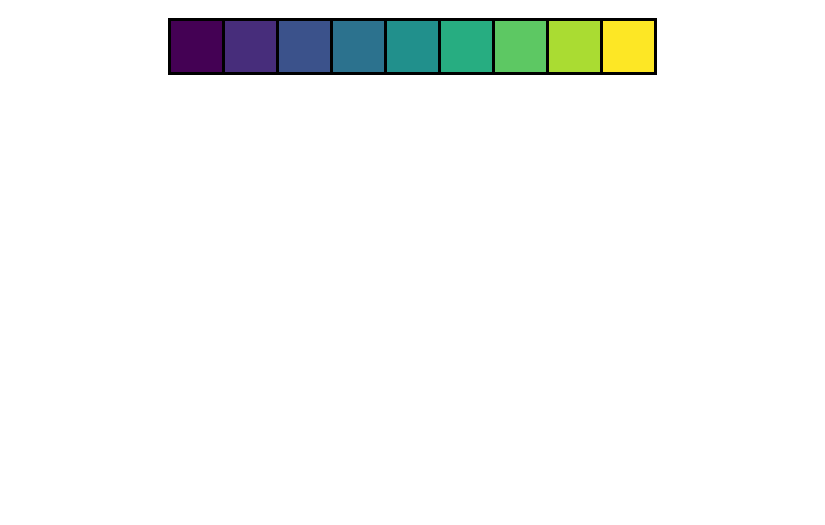
\includegraphics{symbology_files/figure-pdf/unnamed-chunk-9-1.pdf}

}

\caption{Viridis Palette}

\end{figure}%

\chapter{Demonstration Map}\label{demonstration-map}

\begin{Shaded}
\begin{Highlighting}[]
\FunctionTok{library}\NormalTok{(ggplot2) }\CommentTok{\# graphing and mapping}

\FunctionTok{library}\NormalTok{(sf) }\CommentTok{\# simple features}

\NormalTok{city\_boundary }\OtherTok{\textless{}{-}} \FunctionTok{read\_sf}\NormalTok{(}\StringTok{"./shapefiles/AA\_City\_Boundary/AA\_City\_Boundary.shp"}\NormalTok{)}

\NormalTok{clients }\OtherTok{\textless{}{-}} \FunctionTok{read\_sf}\NormalTok{(}\StringTok{"./shapefiles/clients/clients.shp"}\NormalTok{)}

\FunctionTok{ggplot}\NormalTok{(city\_boundary) }\SpecialCharTok{+}
  \FunctionTok{geom\_sf}\NormalTok{(}\AttributeTok{color =} \StringTok{"darkgrey"}\NormalTok{, }\AttributeTok{alpha =}\NormalTok{ .}\DecValTok{5}\NormalTok{) }\SpecialCharTok{+}
  \FunctionTok{geom\_sf}\NormalTok{(}\AttributeTok{data =}\NormalTok{ clients,}
          \FunctionTok{aes}\NormalTok{(}\AttributeTok{color =}\NormalTok{ program), }\CommentTok{\# color = program}
          \AttributeTok{size =} \DecValTok{3}\NormalTok{, }\CommentTok{\# size}
          \AttributeTok{alpha =}\NormalTok{ .}\DecValTok{75}\NormalTok{) }\SpecialCharTok{+} \CommentTok{\# transparency}
  \FunctionTok{labs}\NormalTok{(}\AttributeTok{title =} \StringTok{"Ann Arbor"}\NormalTok{,}
       \AttributeTok{subtitle =} \StringTok{"Locations of Simulated Clients"}\NormalTok{,}
       \AttributeTok{caption =} \StringTok{"Point Color Indicates Program"}\NormalTok{) }\SpecialCharTok{+}
  \FunctionTok{scale\_color\_viridis\_d}\NormalTok{(}\AttributeTok{name=}\StringTok{"Program"}\NormalTok{) }\SpecialCharTok{+} \CommentTok{\# nice viridis colors}
  \FunctionTok{theme\_minimal}\NormalTok{() }\SpecialCharTok{+}
  \FunctionTok{theme}\NormalTok{(}\AttributeTok{plot.title =} \FunctionTok{element\_text}\NormalTok{(}\AttributeTok{size =} \FunctionTok{rel}\NormalTok{(}\DecValTok{2}\NormalTok{)), }
        \AttributeTok{axis.text =} \FunctionTok{element\_text}\NormalTok{(}\AttributeTok{size =} \FunctionTok{rel}\NormalTok{(.}\DecValTok{5}\NormalTok{)),}
        \AttributeTok{legend.position =} \StringTok{"bottom"}\NormalTok{) }
\end{Highlighting}
\end{Shaded}

\includegraphics{symbology_files/figure-pdf/unnamed-chunk-10-1.pdf}

\chapter{\texorpdfstring{Using Data From
\texttt{rnaturalearth}}{Using Data From rnaturalearth}}\label{sec-rnaturalearth}

\texttt{rnaturalearth} is a source library for data various types of
global mapping data.

\section{Call Libraries}\label{call-libraries-2}

\begin{Shaded}
\begin{Highlighting}[]
\FunctionTok{library}\NormalTok{(rnaturalearth) }\CommentTok{\# natural earth data}

\FunctionTok{library}\NormalTok{(ggplot2) }\CommentTok{\# beautiful maps}

\FunctionTok{library}\NormalTok{(dplyr) }\CommentTok{\# data wrangling}

\FunctionTok{library}\NormalTok{(sf) }\CommentTok{\# simple (spatial) features}
\end{Highlighting}
\end{Shaded}

\section{\texorpdfstring{Get \texttt{mapdata} As
\texttt{sf}}{Get mapdata As sf}}\label{get-mapdata-as-sf}

\texttt{ne\_countries} stands for \emph{Natural Earth Countries}.

I use \texttt{ne\_countries()} to create the \texttt{mapdata} dataset as
an \texttt{sf} object (Chapter~\ref{sec-sf}).

\begin{Shaded}
\begin{Highlighting}[]
\NormalTok{mapdata }\OtherTok{\textless{}{-}} \FunctionTok{ne\_countries}\NormalTok{(}\AttributeTok{scale =} \StringTok{"medium"}\NormalTok{, }\CommentTok{\# medium scale}
                        \AttributeTok{returnclass =} \StringTok{"sf"}\NormalTok{) }\CommentTok{\# as sf object}
\end{Highlighting}
\end{Shaded}

\section{Map}\label{map}

\subsection{Simple Basic Map}\label{simple-basic-map}

I make a simple map of this \texttt{sf} object with \texttt{ggplot}
(Chapter~\ref{sec-ggplot-map}).

\begin{Shaded}
\begin{Highlighting}[]
\FunctionTok{ggplot}\NormalTok{(mapdata) }\SpecialCharTok{+} \CommentTok{\# the data I am mapping}
  \FunctionTok{geom\_sf}\NormalTok{() }\CommentTok{\# the geometry I am using}
\end{Highlighting}
\end{Shaded}

\includegraphics{rnaturalearth_files/figure-pdf/unnamed-chunk-3-1.pdf}

\subsection{More Complicated Map}\label{more-complicated-map}

\begin{Shaded}
\begin{Highlighting}[]
\FunctionTok{ggplot}\NormalTok{(mapdata) }\SpecialCharTok{+} \CommentTok{\# the sf data that I am mapping}
  \FunctionTok{geom\_sf}\NormalTok{(}\FunctionTok{aes}\NormalTok{(}\AttributeTok{fill =}\NormalTok{ income\_grp)) }\SpecialCharTok{+} \CommentTok{\# what goes on the map: FILL}
  \FunctionTok{scale\_fill\_viridis\_d}\NormalTok{(}\AttributeTok{name =} \StringTok{"Income Group"}\NormalTok{, }\CommentTok{\# beautiful colors}
                       \AttributeTok{option =} \StringTok{"viridis"}\NormalTok{) }\SpecialCharTok{+}
  \FunctionTok{labs}\NormalTok{(}\AttributeTok{title =} \StringTok{"Countries of the World"}\NormalTok{) }\SpecialCharTok{+} \CommentTok{\# labels}
  \FunctionTok{theme\_minimal}\NormalTok{() }\CommentTok{\# minimal theme}
\end{Highlighting}
\end{Shaded}

\includegraphics{rnaturalearth_files/figure-pdf/unnamed-chunk-4-1.pdf}

\chapter{\texorpdfstring{Using Data From
\texttt{WDI}}{Using Data From WDI}}\label{sec-WDI}

\section{Background}\label{background}

The \href{http://www.worldbank.org/}{World Bank} collects statistical
information from countries around the world. A particularly useful data
set is the \textbf{W}orld \textbf{D}evelopment \textbf{I}ndicators
\href{http://data.worldbank.org/data-catalog/world-development-indicators}{(WDI)}
which are country level statistical information from around the world.

Using \texttt{library(WDI)} you can download indicator data directly
from the World Bank and read it into a data set.

\section{Call Libraries}\label{call-libraries-3}

\begin{Shaded}
\begin{Highlighting}[]
\FunctionTok{library}\NormalTok{(WDI) }\CommentTok{\# for accessing World Bank data}

\FunctionTok{library}\NormalTok{(dplyr) }\CommentTok{\# data wrangling}
\end{Highlighting}
\end{Shaded}

\section{Get Some Data From the World Development Indicators
(WDI)}\label{get-some-data-from-the-world-development-indicators-wdi}

\begin{Shaded}
\begin{Highlighting}[]
\CommentTok{\# get names of specific indicators from WDI Data Catalog}

\NormalTok{WorldBankData }\OtherTok{\textless{}{-}} \FunctionTok{WDI}\NormalTok{(}\AttributeTok{country=}\StringTok{"all"}\NormalTok{, }
                     \AttributeTok{indicator=}\FunctionTok{c}\NormalTok{(}\StringTok{"SI.POV.GINI"}\NormalTok{, }\CommentTok{\# Gini}
                                 \StringTok{"NY.GDP.PCAP.CD"}\NormalTok{, }\CommentTok{\# GDP}
                                 \StringTok{"SE.ADT.LITR.ZS"}\NormalTok{, }\CommentTok{\# adult literacy}
                                 \StringTok{"SP.DYN.LE00.IN"}\NormalTok{, }\CommentTok{\# life expectancy}
                                 \StringTok{"SP.POP.TOTL"}\NormalTok{, }\CommentTok{\# population}
                                 \StringTok{"SN.ITK.DEFC.ZS"}\NormalTok{), }\CommentTok{\# undernourishment}
                     \AttributeTok{start =} \DecValTok{2023}\NormalTok{, }
                     \AttributeTok{end =} \DecValTok{2023}\NormalTok{, }
                     \AttributeTok{extra =} \ConstantTok{TRUE}\NormalTok{) }


\FunctionTok{save}\NormalTok{(WorldBankData, }\AttributeTok{file=}\StringTok{"WorldBankData.RData"}\NormalTok{)}
\end{Highlighting}
\end{Shaded}

\chapter{Rename Some Variables}\label{rename-some-variables}

\begin{Shaded}
\begin{Highlighting}[]
\CommentTok{\# think about renaming some variables with more intuitive names}
\CommentTok{\# e.g....}

\CommentTok{\# rename some variables with dplyr (just copy and paste your indicators)}

\NormalTok{WorldBankData }\OtherTok{\textless{}{-}}\NormalTok{ dplyr}\SpecialCharTok{::}\FunctionTok{rename}\NormalTok{(WorldBankData, }
                        \AttributeTok{GDP =}\NormalTok{ NY.GDP.PCAP.CD,}
                        \AttributeTok{adult\_literacy =}\NormalTok{ SE.ADT.LITR.ZS,}
                        \AttributeTok{life\_expectancy =}\NormalTok{ SP.DYN.LE00.IN, }
                        \AttributeTok{population =}\NormalTok{ SP.POP.TOTL,}
                        \AttributeTok{Gini =}\NormalTok{ SI.POV.GINI,}
                        \AttributeTok{undernourishment =}\NormalTok{ SN.ITK.DEFC.ZS)}

\FunctionTok{save}\NormalTok{(WorldBankData, }\AttributeTok{file=}\StringTok{"WorldBankData.RData"}\NormalTok{)}
\end{Highlighting}
\end{Shaded}

\section{Look At The Data}\label{look-at-the-data}

\begin{Shaded}
\begin{Highlighting}[]
\FunctionTok{load}\NormalTok{(}\StringTok{"WorldBankData.RData"}\NormalTok{) }\CommentTok{\# load the data}

\FunctionTok{head}\NormalTok{(WorldBankData)}
\end{Highlighting}
\end{Shaded}

\begin{verbatim}
                      country iso2c iso3c year status lastupdated Gini      GDP
1                 Afghanistan    AF   AFG 2023         2024-10-24   NA       NA
2 Africa Eastern and Southern    ZH   AFE 2023         2024-10-24   NA 1672.506
3  Africa Western and Central    ZI   AFW 2023         2024-10-24   NA 1584.333
4                     Albania    AL   ALB 2023         2024-10-24   NA 8367.776
5                     Algeria    DZ   DZA 2023         2024-10-24   NA 5260.206
6              American Samoa    AS   ASM 2023         2024-10-24   NA       NA
  adult_literacy life_expectancy population undernourishment
1             NA              NA   42239854               NA
2       73.27511              NA  739108306               NA
3       60.50555              NA  502789511               NA
4             NA              NA    2745972               NA
5             NA              NA   45606480               NA
6             NA              NA      43914               NA
                      region   capital longitude latitude              income
1                 South Asia     Kabul   69.1761  34.5228          Low income
2                 Aggregates                                       Aggregates
3                 Aggregates                                       Aggregates
4      Europe & Central Asia    Tirane   19.8172  41.3317 Upper middle income
5 Middle East & North Africa   Algiers   3.05097  36.7397 Lower middle income
6        East Asia & Pacific Pago Pago  -170.691 -14.2846 Upper middle income
         lending
1            IDA
2     Aggregates
3     Aggregates
4           IBRD
5           IBRD
6 Not classified
\end{verbatim}

\part{Mapping With \texttt{ggplot}}

\chapter{\texorpdfstring{Making Maps with
\texttt{ggplot}}{Making Maps with ggplot}}\label{sec-ggplot-map}

\section{Call the libraries}\label{call-the-libraries-1}

\begin{Shaded}
\begin{Highlighting}[]
\FunctionTok{library}\NormalTok{(ggplot2) }\CommentTok{\# beautiful graphs}

\FunctionTok{library}\NormalTok{(dplyr) }\CommentTok{\# data wrangling}

\FunctionTok{library}\NormalTok{(sf) }\CommentTok{\# simple (spatial) features}

\FunctionTok{library}\NormalTok{(readr) }\CommentTok{\# import csv}
\end{Highlighting}
\end{Shaded}

\section{\texorpdfstring{Use \texttt{read\_sf} To Open
Shapefiles}{Use read\_sf To Open Shapefiles}}\label{use-read_sf-to-open-shapefiles}

\begin{quote}
Getting the directory and filename right is important.
\end{quote}

\begin{Shaded}
\begin{Highlighting}[]
\NormalTok{city\_boundary }\OtherTok{\textless{}{-}} \FunctionTok{read\_sf}\NormalTok{(}\StringTok{"./shapefiles/AA\_City\_Boundary/AA\_City\_Boundary.shp"}\NormalTok{)}

\NormalTok{buildings }\OtherTok{\textless{}{-}} \FunctionTok{read\_sf}\NormalTok{(}\StringTok{"./shapefiles/AA\_Building\_Footprints/AA\_Building\_Footprints.shp"}\NormalTok{)}

\NormalTok{trees }\OtherTok{\textless{}{-}} \FunctionTok{read\_sf}\NormalTok{(}\StringTok{"./shapefiles/a2trees/AA\_Trees.shp"}\NormalTok{)}

\NormalTok{parks }\OtherTok{\textless{}{-}} \FunctionTok{read\_sf}\NormalTok{(}\StringTok{"./shapefiles/AA\_Parks/AA\_Parks.shp"}\NormalTok{)}

\NormalTok{university }\OtherTok{\textless{}{-}} \FunctionTok{read\_sf}\NormalTok{(}\StringTok{"./shapefiles/AA\_University/AA\_University.shp"}\NormalTok{)}

\NormalTok{WashtenawRoads }\OtherTok{\textless{}{-}} \FunctionTok{read\_sf}\NormalTok{(}\StringTok{"./shapefiles/Roads/RoadCenterlines.shp"}\NormalTok{)}

\NormalTok{AnnArborRoads }\OtherTok{\textless{}{-}} \FunctionTok{st\_crop}\NormalTok{(WashtenawRoads, }
\NormalTok{                         city\_boundary) }\CommentTok{\# crop to only get A2 roads}
\end{Highlighting}
\end{Shaded}

\begin{verbatim}
Warning: attribute variables are assumed to be spatially constant throughout
all geometries
\end{verbatim}

\begin{Shaded}
\begin{Highlighting}[]
\CommentTok{\# watersheds \textless{}{-} read\_sf("../shapefiles/watersheds/Watersheds.shp")}
\end{Highlighting}
\end{Shaded}

\section{\texorpdfstring{Use \texttt{ggplot} to Make The
Map}{Use ggplot to Make The Map}}\label{use-ggplot-to-make-the-map}

\begin{Shaded}
\begin{Highlighting}[]
\CommentTok{\# NB RE Macs: the plotting device on Macs can be very slow}
\CommentTok{\# we notice this with all the detail that is involved in maps}
\CommentTok{\# maps can be REALLY slow on Macs}
\CommentTok{\# so{-}{-}inconveniently{-}{-}we write directly to PDF on a Mac}
\CommentTok{\# and don\textquotesingle{}t see the graph in our RStudio window}
\CommentTok{\# we have to manually open the PDF to see the created map}

\CommentTok{\# Apparently, the first layer is important for setting the CRS of the map}

\CommentTok{\# pdf("./mapping/ggplot{-}map{-}test.pdf") \# open PDF device (uncomment on Mac)}

\CommentTok{\# dev.off() \# turn off PDF device (uncomment on Mac)}
\end{Highlighting}
\end{Shaded}

\begin{Shaded}
\begin{Highlighting}[]
\FunctionTok{ggplot}\NormalTok{(city\_boundary) }\SpecialCharTok{+}
  \CommentTok{\# geom\_sf(data = buildings,}
  \CommentTok{\#         fill = "lightgrey") +}
  \FunctionTok{geom\_sf}\NormalTok{(}\AttributeTok{data =}\NormalTok{ AnnArborRoads, }
          \AttributeTok{color =} \StringTok{"lightgrey"}\NormalTok{) }\SpecialCharTok{+}
  \FunctionTok{geom\_sf}\NormalTok{(}\AttributeTok{color =} \StringTok{"darkgrey"}\NormalTok{, }\AttributeTok{alpha =}\NormalTok{ .}\DecValTok{5}\NormalTok{) }\SpecialCharTok{+}
  \FunctionTok{geom\_sf}\NormalTok{(}\AttributeTok{data =}\NormalTok{ university, }
          \FunctionTok{aes}\NormalTok{(}\AttributeTok{fill =} \StringTok{"university or college"}\NormalTok{), }
          \AttributeTok{alpha =}\NormalTok{ .}\DecValTok{75}\NormalTok{) }\SpecialCharTok{+} 
  \FunctionTok{geom\_sf}\NormalTok{(}\AttributeTok{data =}\NormalTok{ parks, }
          \AttributeTok{alpha =}\NormalTok{ .}\DecValTok{75}\NormalTok{,}
          \FunctionTok{aes}\NormalTok{(}\AttributeTok{fill =} \StringTok{"parks"}\NormalTok{)) }\SpecialCharTok{+}
  \CommentTok{\# geom\_sf(data = trees, }
  \CommentTok{\#         size = .1,}
  \CommentTok{\#         color = "darkgreen") +}
  \FunctionTok{labs}\NormalTok{(}\AttributeTok{title =} \StringTok{"Ann Arbor"}\NormalTok{) }\SpecialCharTok{+}
  \FunctionTok{scale\_color\_viridis\_d}\NormalTok{() }\SpecialCharTok{+}
  \FunctionTok{scale\_fill\_manual}\NormalTok{(}\AttributeTok{name=}\StringTok{""}\NormalTok{,}
                    \AttributeTok{values =} \FunctionTok{c}\NormalTok{(}\StringTok{"darkgreen"}\NormalTok{, }\StringTok{"navy"}\NormalTok{)) }\SpecialCharTok{+}
  \FunctionTok{theme\_minimal}\NormalTok{() }\SpecialCharTok{+}
  \FunctionTok{theme}\NormalTok{(}\AttributeTok{plot.title =} \FunctionTok{element\_text}\NormalTok{(}\AttributeTok{size =} \FunctionTok{rel}\NormalTok{(}\DecValTok{2}\NormalTok{)), }
        \AttributeTok{axis.text =} \FunctionTok{element\_text}\NormalTok{(}\AttributeTok{size =} \FunctionTok{rel}\NormalTok{(.}\DecValTok{5}\NormalTok{)),}
        \AttributeTok{legend.position =} \StringTok{"bottom"}\NormalTok{) }
\end{Highlighting}
\end{Shaded}

\includegraphics{ggplot-map_files/figure-pdf/unnamed-chunk-4-1.pdf}

\chapter{Merge Shapefiles With External Data}\label{sec-merging}

\section{Introduction}\label{introduction-4}

A common task in mapping is that we have a \emph{shapefile}
(Chapter~\ref{sec-shapefiles}) or \texttt{sf} object
(Chapter~\ref{sec-sf}) of map data, but we want to merge in some
\emph{external data} from another source so that we can map that
\emph{external data}.

Often we want to use different colors to map that external data
(Chapter~\ref{sec-symbology}).

Here, I use an \texttt{sf} object (Chapter~\ref{sec-sf}) of countries of
the world (Chapter~\ref{sec-rnaturalearth}), and merge that data with
data from the World Bank World Development Indicators
(Chapter~\ref{sec-WDI}).

This tutorial builds upon another tutorial on Mapping with
\texttt{ggplot}(Chapter~\ref{sec-ggplot-map})

\section{Call Libraries}\label{call-libraries-4}

\begin{Shaded}
\begin{Highlighting}[]
\FunctionTok{library}\NormalTok{(rnaturalearth) }\CommentTok{\# natural earth data}

\FunctionTok{library}\NormalTok{(sf) }\CommentTok{\# simple (spatial) features}

\FunctionTok{library}\NormalTok{(ggplot2) }\CommentTok{\# beautiful plots}

\FunctionTok{library}\NormalTok{(dplyr) }\CommentTok{\# data wrangling and joins}
\end{Highlighting}
\end{Shaded}

\section{Get Map Data on Countries of the
World}\label{get-map-data-on-countries-of-the-world}

I am using the \texttt{rnaturalearth} package to get map data on
countries of the world. I read this data into an object called
\texttt{world}.

\begin{Shaded}
\begin{Highlighting}[]
\NormalTok{mapdata }\OtherTok{\textless{}{-}} \FunctionTok{ne\_countries}\NormalTok{(}\AttributeTok{scale =} \StringTok{"medium"}\NormalTok{, }\CommentTok{\# medium scale}
                        \AttributeTok{returnclass =} \StringTok{"sf"}\NormalTok{) }\CommentTok{\# as sf object}
\end{Highlighting}
\end{Shaded}

\section{Make a Map Without Data}\label{make-a-map-without-data}

I map the data with \texttt{ggplot}, and the special \texttt{geom},
\texttt{geom\_sf}.

\begin{Shaded}
\begin{Highlighting}[]
\FunctionTok{ggplot}\NormalTok{(mapdata) }\SpecialCharTok{+} 
  \FunctionTok{geom\_sf}\NormalTok{() }\SpecialCharTok{+}
  \FunctionTok{labs}\NormalTok{(}\AttributeTok{title =} \StringTok{"Demonstration Map With No Data"}\NormalTok{)}
\end{Highlighting}
\end{Shaded}

\includegraphics{merge-with-external-data_files/figure-pdf/unnamed-chunk-3-1.pdf}

\section{Get External Data}\label{get-external-data}

Here I load the World Bank Data (Chapter~\ref{sec-WDI}).

\begin{Shaded}
\begin{Highlighting}[]
\FunctionTok{load}\NormalTok{(}\StringTok{"WorldBankData.Rdata"}\NormalTok{)}

\FunctionTok{head}\NormalTok{(WorldBankData) }\CommentTok{\# replay data set}
\end{Highlighting}
\end{Shaded}

\begin{verbatim}
                      country iso2c iso3c year status lastupdated Gini      GDP
1                 Afghanistan    AF   AFG 2023         2024-10-24   NA       NA
2 Africa Eastern and Southern    ZH   AFE 2023         2024-10-24   NA 1672.506
3  Africa Western and Central    ZI   AFW 2023         2024-10-24   NA 1584.333
4                     Albania    AL   ALB 2023         2024-10-24   NA 8367.776
5                     Algeria    DZ   DZA 2023         2024-10-24   NA 5260.206
6              American Samoa    AS   ASM 2023         2024-10-24   NA       NA
  adult_literacy life_expectancy population undernourishment
1             NA              NA   42239854               NA
2       73.27511              NA  739108306               NA
3       60.50555              NA  502789511               NA
4             NA              NA    2745972               NA
5             NA              NA   45606480               NA
6             NA              NA      43914               NA
                      region   capital longitude latitude              income
1                 South Asia     Kabul   69.1761  34.5228          Low income
2                 Aggregates                                       Aggregates
3                 Aggregates                                       Aggregates
4      Europe & Central Asia    Tirane   19.8172  41.3317 Upper middle income
5 Middle East & North Africa   Algiers   3.05097  36.7397 Lower middle income
6        East Asia & Pacific Pago Pago  -170.691 -14.2846 Upper middle income
         lending
1            IDA
2     Aggregates
3     Aggregates
4           IBRD
5           IBRD
6 Not classified
\end{verbatim}

\section{Join Data to Shapefile}\label{join-data-to-shapefile}

I use \texttt{left\_join} from the \texttt{dplyr} package to merge the
spatial data in \texttt{world} with \texttt{externaldata}.

\texttt{left\_join} is a function that keeps all observations in the
data on the left (the shapefile), and only those matching observations
in the data on the right (the external data), which is usually what I
want in mapping.

I need a unique identifier for my rows of data, so here I use
\texttt{iso\_a3}, a unique 3 letter identifier for countries of the
world.

First I need to make a copy of a variable in \texttt{WorldBankData} with
a new name so that the identifiers will match exactly.

\begin{Shaded}
\begin{Highlighting}[]
\NormalTok{WorldBankData}\SpecialCharTok{$}\NormalTok{iso\_a3 }\OtherTok{\textless{}{-}}\NormalTok{ WorldBankData}\SpecialCharTok{$}\NormalTok{iso3c }
\end{Highlighting}
\end{Shaded}

Then I merge the data using \texttt{left\_join}.

\begin{Shaded}
\begin{Highlighting}[]
\NormalTok{newdata }\OtherTok{\textless{}{-}} \FunctionTok{left\_join}\NormalTok{(mapdata, }\CommentTok{\# map data}
\NormalTok{                     WorldBankData, }\CommentTok{\# table of indicators}
                     \AttributeTok{by =} \StringTok{"iso\_a3"}\NormalTok{) }\CommentTok{\# join by}
\end{Highlighting}
\end{Shaded}

\section{Make a Map With The Data}\label{make-a-map-with-the-data}

Once I have the merged data, it is easy to map it with \texttt{ggplot}
and \texttt{geom\_sf}. Note that I need to specify an \texttt{aes}thetic
for \texttt{geom\_sf}. Here \texttt{GDP} is the \emph{fill} color for
countries on the map.

\begin{quote}
Data could also be mapped with another package like \texttt{leaflet}
(Chapter~\ref{sec-leaflet}).
\end{quote}

\begin{Shaded}
\begin{Highlighting}[]
\FunctionTok{ggplot}\NormalTok{(newdata) }\SpecialCharTok{+}
  \FunctionTok{geom\_sf}\NormalTok{(}\FunctionTok{aes}\NormalTok{(}\AttributeTok{fill =}\NormalTok{ GDP)) }\SpecialCharTok{+} \CommentTok{\# adding a fill aesthetic}
  \FunctionTok{scale\_fill\_viridis\_c}\NormalTok{(}\AttributeTok{na.value =} \StringTok{"grey97"}\NormalTok{, }\CommentTok{\# value for NA}
                       \AttributeTok{option =} \StringTok{"viridis"}\NormalTok{) }\SpecialCharTok{+} \CommentTok{\# viridis colors}
  \FunctionTok{labs}\NormalTok{(}\AttributeTok{title =} \StringTok{"Demonstration Map With Merged Data"}\NormalTok{) }\SpecialCharTok{+}
  \FunctionTok{theme\_minimal}\NormalTok{() }\CommentTok{\# better theme}
\end{Highlighting}
\end{Shaded}

\includegraphics{merge-with-external-data_files/figure-pdf/unnamed-chunk-7-1.pdf}

\chapter{\texorpdfstring{Making Maps With \texttt{ggplot} Using Location
Data}{Making Maps With ggplot Using Location Data}}\label{sec-location-data}

\section{Call Libraries}\label{call-libraries-5}

\begin{Shaded}
\begin{Highlighting}[]
\FunctionTok{library}\NormalTok{(readr) }\CommentTok{\# read CSV}

\FunctionTok{library}\NormalTok{(dplyr) }\CommentTok{\# data wrangling}

\FunctionTok{library}\NormalTok{(sf) }\CommentTok{\# simple features}

\FunctionTok{library}\NormalTok{(ggplot2) }\CommentTok{\# maps}
\end{Highlighting}
\end{Shaded}

\section{\texorpdfstring{Use \texttt{read\_csv} to Read Text File with
Client
Data}{Use read\_csv to Read Text File with Client Data}}\label{use-read_csv-to-read-text-file-with-client-data}

\begin{Shaded}
\begin{Highlighting}[]
\NormalTok{clients }\OtherTok{\textless{}{-}} \FunctionTok{read\_csv}\NormalTok{(}\StringTok{"./location{-}data/clients.csv"}\NormalTok{)}
\end{Highlighting}
\end{Shaded}

\section{Only Clients in Ann Arbor
Area}\label{only-clients-in-ann-arbor-area}

\begin{Shaded}
\begin{Highlighting}[]
\NormalTok{clients }\OtherTok{\textless{}{-}}\NormalTok{ clients }\SpecialCharTok{\%\textgreater{}\%} 
  \FunctionTok{filter}\NormalTok{(latitude }\SpecialCharTok{\textless{}=} \FloatTok{42.33} \SpecialCharTok{\&}
\NormalTok{           latitude }\SpecialCharTok{\textgreater{}=} \FloatTok{42.22} \SpecialCharTok{\&}
\NormalTok{           longitude }\SpecialCharTok{\textgreater{}=} \SpecialCharTok{{-}}\FloatTok{83.8} \SpecialCharTok{\&}
\NormalTok{           longitude }\SpecialCharTok{\textless{}=} \SpecialCharTok{{-}}\FloatTok{83.65}\NormalTok{)}
\end{Highlighting}
\end{Shaded}

\section{\texorpdfstring{Convert Clients to \texttt{sf} Object While
Indicating \emph{Coordinate Reference System}
(CRS)}{Convert Clients to sf Object While Indicating Coordinate Reference System (CRS)}}\label{convert-clients-to-sf-object-while-indicating-coordinate-reference-system-crs}

\begin{Shaded}
\begin{Highlighting}[]
\NormalTok{point }\OtherTok{\textless{}{-}} \FunctionTok{st\_as\_sf}\NormalTok{(clients, }
                  \AttributeTok{coords =} \FunctionTok{c}\NormalTok{(}\StringTok{"longitude"}\NormalTok{, }\StringTok{"latitude"}\NormalTok{), }
                  \AttributeTok{crs =} \DecValTok{4269}\NormalTok{) }\CommentTok{\# A2 is NAD1983}

\CommentTok{\# write to shapefile}

\FunctionTok{st\_write}\NormalTok{(point, }
         \StringTok{"./shapefiles/clients/clients.shp"}\NormalTok{,}
         \AttributeTok{append =} \ConstantTok{FALSE}\NormalTok{) }\CommentTok{\# replace; don\textquotesingle{}t append}
\end{Highlighting}
\end{Shaded}

\section{Read in Shapefile(s)}\label{read-in-shapefiles}

\begin{Shaded}
\begin{Highlighting}[]
\NormalTok{city\_boundary }\OtherTok{\textless{}{-}} \FunctionTok{read\_sf}\NormalTok{(}\StringTok{"./shapefiles/AA\_City\_Boundary/AA\_City\_Boundary.shp"}\NormalTok{)}

\NormalTok{WashtenawRoads }\OtherTok{\textless{}{-}} \FunctionTok{read\_sf}\NormalTok{(}\StringTok{"./shapefiles/Roads/RoadCenterlines.shp"}\NormalTok{)}

\NormalTok{AnnArborRoads }\OtherTok{\textless{}{-}} \FunctionTok{st\_crop}\NormalTok{(WashtenawRoads, }
\NormalTok{                         city\_boundary) }\CommentTok{\# crop to only get A2 roads}
\end{Highlighting}
\end{Shaded}

\section{Map}\label{map-1}

\begin{Shaded}
\begin{Highlighting}[]
\FunctionTok{ggplot}\NormalTok{(city\_boundary) }\SpecialCharTok{+}
  \FunctionTok{geom\_sf}\NormalTok{(}\AttributeTok{alpha =}\NormalTok{ .}\DecValTok{5}\NormalTok{) }\SpecialCharTok{+}
  \FunctionTok{geom\_sf}\NormalTok{(}\AttributeTok{data =}\NormalTok{ AnnArborRoads, }
          \AttributeTok{color =} \StringTok{"darkgrey"}\NormalTok{) }\SpecialCharTok{+}
  \FunctionTok{geom\_sf}\NormalTok{(}\AttributeTok{data =}\NormalTok{ point,}
          \FunctionTok{aes}\NormalTok{(}\AttributeTok{color =}\NormalTok{ program),}
          \AttributeTok{size =} \DecValTok{3}\NormalTok{) }\SpecialCharTok{+}
\FunctionTok{labs}\NormalTok{(}\AttributeTok{title =} \StringTok{"Ann Arbor"}\NormalTok{,}
     \AttributeTok{subtitle =} \StringTok{"Location of Program Clients"}\NormalTok{) }\SpecialCharTok{+}
  \FunctionTok{scale\_color\_viridis\_d}\NormalTok{() }\SpecialCharTok{+}
  \FunctionTok{scale\_fill\_viridis\_d}\NormalTok{() }\SpecialCharTok{+}
  \FunctionTok{theme\_minimal}\NormalTok{() }\SpecialCharTok{+}
  \FunctionTok{theme}\NormalTok{(}\AttributeTok{plot.title =} \FunctionTok{element\_text}\NormalTok{(}\AttributeTok{size =} \FunctionTok{rel}\NormalTok{(}\DecValTok{2}\NormalTok{)), }
        \AttributeTok{axis.text =} \FunctionTok{element\_text}\NormalTok{(}\AttributeTok{size =} \FunctionTok{rel}\NormalTok{(.}\DecValTok{5}\NormalTok{)),}
        \AttributeTok{legend.position =} \StringTok{"bottom"}\NormalTok{) }
\end{Highlighting}
\end{Shaded}

\includegraphics{location-data_files/figure-pdf/unnamed-chunk-6-1.pdf}

\part{More Advanced GIS Concepts}

\chapter{Geocoding}\label{sec-geocoding}

\section{Call Libraries}\label{call-libraries-6}

\begin{Shaded}
\begin{Highlighting}[]
\FunctionTok{library}\NormalTok{(tidygeocoder) }\CommentTok{\# geocoding}
\end{Highlighting}
\end{Shaded}

\begin{verbatim}
Warning: package 'tidygeocoder' was built under R version 4.4.2
\end{verbatim}

\begin{Shaded}
\begin{Highlighting}[]
\FunctionTok{library}\NormalTok{(dplyr) }\CommentTok{\# for \%\textgreater{}\% operator}

\FunctionTok{library}\NormalTok{(readr) }\CommentTok{\# import CSV}

\FunctionTok{library}\NormalTok{(DT) }\CommentTok{\# nice tables}
\end{Highlighting}
\end{Shaded}

\section{Get Data To Be Geocoded}\label{get-data-to-be-geocoded}

\begin{Shaded}
\begin{Highlighting}[]
\NormalTok{simulated\_address\_data }\OtherTok{\textless{}{-}} \FunctionTok{read\_csv}\NormalTok{(}\StringTok{"simulated{-}address{-}data/simulated{-}address{-}data.csv"}\NormalTok{)}

\NormalTok{DT}\SpecialCharTok{::}\FunctionTok{datatable}\NormalTok{(simulated\_address\_data,}
              \AttributeTok{extensions =} \StringTok{\textquotesingle{}Buttons\textquotesingle{}}\NormalTok{, }
              \AttributeTok{options =} \FunctionTok{list}\NormalTok{(}
                \AttributeTok{dom =} \StringTok{\textquotesingle{}Bfrtip\textquotesingle{}}\NormalTok{,}
                \AttributeTok{buttons =} \FunctionTok{c}\NormalTok{(}\StringTok{\textquotesingle{}copy\textquotesingle{}}\NormalTok{, }
                            \StringTok{\textquotesingle{}csv\textquotesingle{}}\NormalTok{, }
                            \StringTok{\textquotesingle{}print\textquotesingle{}}\NormalTok{))) }\CommentTok{\# nice table}
\end{Highlighting}
\end{Shaded}

\includegraphics{geocoding_files/figure-pdf/unnamed-chunk-2-1.pdf}

\section{Concatenate Addresses}\label{concatenate-addresses}

\begin{Shaded}
\begin{Highlighting}[]
\NormalTok{simulated\_address\_data}\SpecialCharTok{$}\NormalTok{address }\OtherTok{\textless{}{-}} \FunctionTok{paste}\NormalTok{(simulated\_address\_data}\SpecialCharTok{$}\NormalTok{street,}
                                        \StringTok{", "}\NormalTok{,}
\NormalTok{                                        simulated\_address\_data}\SpecialCharTok{$}\NormalTok{city,}
                                        \StringTok{", "}\NormalTok{,}
\NormalTok{                                        simulated\_address\_data}\SpecialCharTok{$}\NormalTok{state)}

\NormalTok{DT}\SpecialCharTok{::}\FunctionTok{datatable}\NormalTok{(simulated\_address\_data,}
              \AttributeTok{extensions =} \StringTok{\textquotesingle{}Buttons\textquotesingle{}}\NormalTok{, }
              \AttributeTok{options =} \FunctionTok{list}\NormalTok{(}
                \AttributeTok{dom =} \StringTok{\textquotesingle{}Bfrtip\textquotesingle{}}\NormalTok{,}
                \AttributeTok{buttons =} \FunctionTok{c}\NormalTok{(}\StringTok{\textquotesingle{}copy\textquotesingle{}}\NormalTok{, }
                            \StringTok{\textquotesingle{}csv\textquotesingle{}}\NormalTok{, }
                            \StringTok{\textquotesingle{}print\textquotesingle{}}\NormalTok{))) }\CommentTok{\# nice table}
\end{Highlighting}
\end{Shaded}

\includegraphics{geocoding_files/figure-pdf/unnamed-chunk-3-1.pdf}

\section{Geocode}\label{geocode}

\begin{tcolorbox}[enhanced jigsaw, opacityback=0, colback=white, toprule=.15mm, colframe=quarto-callout-caution-color-frame, bottomrule=.15mm, title=\textcolor{quarto-callout-caution-color}{\faFire}\hspace{0.5em}{Caution}, coltitle=black, toptitle=1mm, bottomtitle=1mm, arc=.35mm, breakable, colbacktitle=quarto-callout-caution-color!10!white, left=2mm, rightrule=.15mm, titlerule=0mm, leftrule=.75mm, opacitybacktitle=0.6]

ArcGIS geocoding has LOW success rate with this data. You will want to
find a process with HIGH success rate.

\end{tcolorbox}

\begin{tcolorbox}[enhanced jigsaw, opacityback=0, colback=white, toprule=.15mm, colframe=quarto-callout-tip-color-frame, bottomrule=.15mm, title=\textcolor{quarto-callout-tip-color}{\faLightbulb}\hspace{0.5em}{Tip}, coltitle=black, toptitle=1mm, bottomtitle=1mm, arc=.35mm, breakable, colbacktitle=quarto-callout-tip-color!10!white, left=2mm, rightrule=.15mm, titlerule=0mm, leftrule=.75mm, opacitybacktitle=0.6]

You could also try batchgeo -\textgreater{} KML -\textgreater{}
Latitude/Longitude

\end{tcolorbox}

\begin{Shaded}
\begin{Highlighting}[]
\NormalTok{geocoded\_data }\OtherTok{\textless{}{-}}\NormalTok{ simulated\_address\_data }\SpecialCharTok{\%\textgreater{}\%} 
\NormalTok{  tidygeocoder}\SpecialCharTok{::}\FunctionTok{geocode}\NormalTok{(address, }
                        \AttributeTok{method =} \StringTok{\textquotesingle{}arcgis\textquotesingle{}}\NormalTok{, }
                        \AttributeTok{lat =}\NormalTok{ latitude, }
                        \AttributeTok{long =}\NormalTok{ longitude)}
\end{Highlighting}
\end{Shaded}

\begin{verbatim}
Passing 3 addresses to the ArcGIS single address geocoder
\end{verbatim}

\begin{verbatim}
Query completed in: 2.2 seconds
\end{verbatim}

\begin{Shaded}
\begin{Highlighting}[]
\NormalTok{DT}\SpecialCharTok{::}\FunctionTok{datatable}\NormalTok{(geocoded\_data,}
              \AttributeTok{extensions =} \StringTok{\textquotesingle{}Buttons\textquotesingle{}}\NormalTok{, }
              \AttributeTok{options =} \FunctionTok{list}\NormalTok{(}
                \AttributeTok{dom =} \StringTok{\textquotesingle{}Bfrtip\textquotesingle{}}\NormalTok{,}
                \AttributeTok{buttons =} \FunctionTok{c}\NormalTok{(}\StringTok{\textquotesingle{}copy\textquotesingle{}}\NormalTok{, }
                            \StringTok{\textquotesingle{}csv\textquotesingle{}}\NormalTok{, }
                            \StringTok{\textquotesingle{}print\textquotesingle{}}\NormalTok{))) }\CommentTok{\# nice table}
\end{Highlighting}
\end{Shaded}

\includegraphics{geocoding_files/figure-pdf/unnamed-chunk-4-1.pdf}

\begin{tcolorbox}[enhanced jigsaw, opacityback=0, colback=white, toprule=.15mm, colframe=quarto-callout-important-color-frame, bottomrule=.15mm, title=\textcolor{quarto-callout-important-color}{\faExclamation}\hspace{0.5em}{Geocoding Can Make Errors!}, coltitle=black, toptitle=1mm, bottomtitle=1mm, arc=.35mm, breakable, colbacktitle=quarto-callout-important-color!10!white, left=2mm, rightrule=.15mm, titlerule=0mm, leftrule=.75mm, opacitybacktitle=0.6]

NB that for whatever reason--perhaps because there is no address
information--the geocoder has made a mistake: Agency Z has been placed
in the Southern Hemisphere. Geocoding can be an error prone process and
requires careful inspection of your tabular and mapped data.

A geocoder may also be unable to geocode some of your data. Low success
rates are not uncommon, and you may have to work hard to ensure that the
majority, or all, of your data are geocoded.

\end{tcolorbox}

\begin{quote}
Geocoded data can then be mapped using procedures outlined in
Chapter~\ref{sec-location-data}.
\end{quote}

\chapter{\texorpdfstring{\texttt{cartogram}}{cartogram}}\label{cartogram}

A \emph{cartogram} is a map where the areas of different regions are
distorted (increased in size; decreased in size) by the value of some
quantitative variable.

\section{Call Libraries}\label{call-libraries-7}

\begin{Shaded}
\begin{Highlighting}[]
\FunctionTok{library}\NormalTok{(rnaturalearth) }\CommentTok{\# natural earth data}

\FunctionTok{library}\NormalTok{(ggplot2) }\CommentTok{\# beautiful maps}

\FunctionTok{library}\NormalTok{(dplyr) }\CommentTok{\# data wrangling}

\FunctionTok{library}\NormalTok{(sf) }\CommentTok{\# simple (spatial) features}

\FunctionTok{library}\NormalTok{(cartogram) }\CommentTok{\# cartograms!}
\end{Highlighting}
\end{Shaded}

\section{Remove Scientific Notation}\label{remove-scientific-notation}

\begin{Shaded}
\begin{Highlighting}[]
\FunctionTok{options}\NormalTok{(}\AttributeTok{scipen =} \DecValTok{999}\NormalTok{) }\CommentTok{\# high \textquotesingle{}penalty\textquotesingle{} for scientific notation}
\end{Highlighting}
\end{Shaded}

\section{\texorpdfstring{Get Map Data From
\texttt{rnaturalearth}}{Get Map Data From rnaturalearth}}\label{get-map-data-from-rnaturalearth}

\begin{Shaded}
\begin{Highlighting}[]
\NormalTok{mapdata }\OtherTok{\textless{}{-}} \FunctionTok{ne\_countries}\NormalTok{(}\AttributeTok{scale =} \StringTok{"medium"}\NormalTok{, }\CommentTok{\# medium scale}
                        \AttributeTok{returnclass =} \StringTok{"sf"}\NormalTok{)  }\CommentTok{\# as sf object}
\end{Highlighting}
\end{Shaded}

\section{Make A Basic Map}\label{make-a-basic-map}

We make a basic map, reading it into an object called \texttt{mymap.} We
then \emph{replay} \texttt{mymap.}

\begin{Shaded}
\begin{Highlighting}[]
\NormalTok{mymap }\OtherTok{\textless{}{-}} \FunctionTok{ggplot}\NormalTok{(mapdata) }\SpecialCharTok{+} \CommentTok{\# the data I am mapping}
  \FunctionTok{geom\_sf}\NormalTok{() }\CommentTok{\# the geometry I am using}

\NormalTok{mymap }\CommentTok{\# replay my map}
\end{Highlighting}
\end{Shaded}

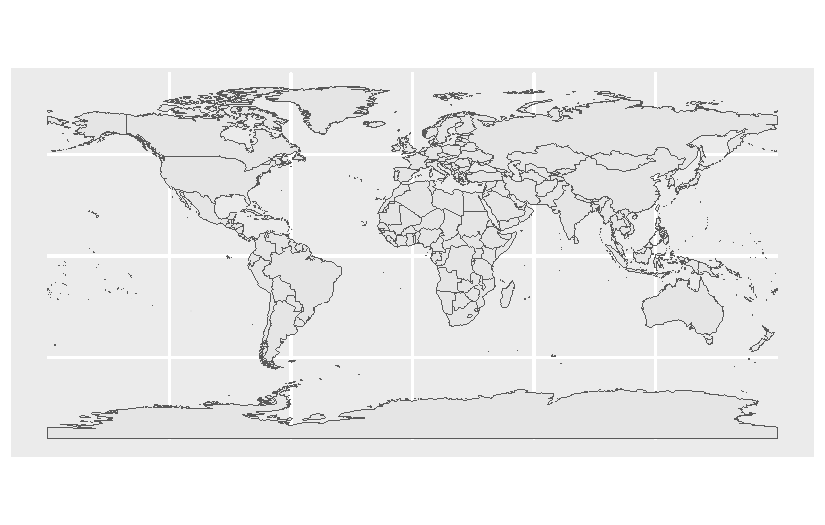
\includegraphics{cartogram_files/figure-pdf/unnamed-chunk-4-1.pdf}

\section{Make And Plot The Cartogram}\label{make-and-plot-the-cartogram}

\subsection{Project The Cartogram
Data}\label{project-the-cartogram-data}

\begin{tcolorbox}[enhanced jigsaw, opacityback=0, colback=white, toprule=.15mm, colframe=quarto-callout-tip-color-frame, bottomrule=.15mm, title=\textcolor{quarto-callout-tip-color}{\faLightbulb}\hspace{0.5em}{Tip}, coltitle=black, toptitle=1mm, bottomtitle=1mm, arc=.35mm, breakable, colbacktitle=quarto-callout-tip-color!10!white, left=2mm, rightrule=.15mm, titlerule=0mm, leftrule=.75mm, opacitybacktitle=0.6]

\texttt{cartogram} requires \emph{projected} data
(Chapter~\ref{sec-projections}), so we need to project the data with
\texttt{st\_transform}. A number of projections, including the
\emph{Mercator} and \emph{Mollweide} projections are possibilities. You
may need to experiment with a number of projections to see which ones
work best in any particular cartogram.

\end{tcolorbox}

\begin{Shaded}
\begin{Highlighting}[]
\NormalTok{mapdata\_proj }\OtherTok{\textless{}{-}} \FunctionTok{st\_transform}\NormalTok{(mapdata,}
                             \DecValTok{3857}\NormalTok{) }\CommentTok{\# Mercator}

\CommentTok{\# mapdata\_proj \textless{}{-} st\_transform(mapdata, }
\CommentTok{\#                              crs = "+proj=moll") \# Mollweide}
\end{Highlighting}
\end{Shaded}

\subsection{Plot The Projected Data}\label{plot-the-projected-data}

\begin{Shaded}
\begin{Highlighting}[]
\FunctionTok{ggplot}\NormalTok{(mapdata\_proj) }\SpecialCharTok{+} 
  \FunctionTok{geom\_sf}\NormalTok{() }\CommentTok{\# plot projected data}
\end{Highlighting}
\end{Shaded}

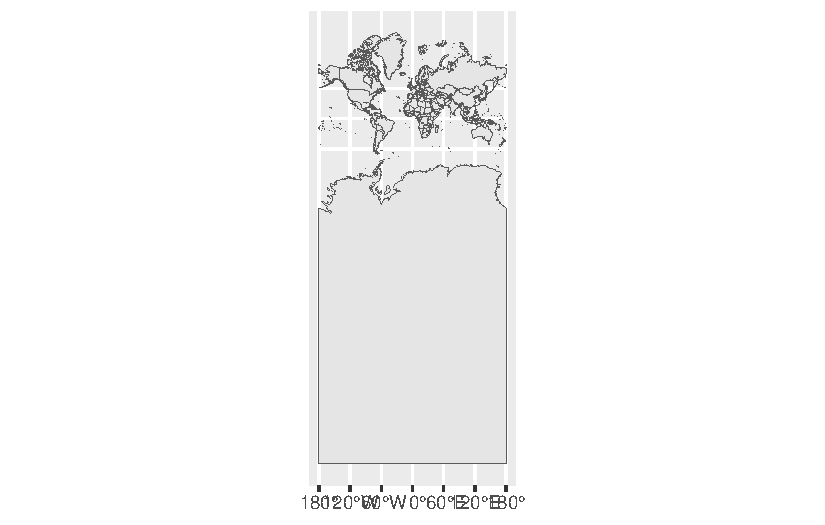
\includegraphics{cartogram_files/figure-pdf/unnamed-chunk-6-1.pdf}

\begin{tcolorbox}[enhanced jigsaw, opacityback=0, colback=white, toprule=.15mm, colframe=quarto-callout-tip-color-frame, bottomrule=.15mm, title=\textcolor{quarto-callout-tip-color}{\faLightbulb}\hspace{0.5em}{Why Does Antarctica Look So Strange? How To Fix This?}, coltitle=black, toptitle=1mm, bottomtitle=1mm, arc=.35mm, breakable, colbacktitle=quarto-callout-tip-color!10!white, left=2mm, rightrule=.15mm, titlerule=0mm, leftrule=.75mm, opacitybacktitle=0.6]

In some projections, especially the \emph{Mercator} projection,
Antartica looks strange.

The key is to run this \texttt{dplyr} code to remove Antarctica.

\begin{Shaded}
\begin{Highlighting}[]
\NormalTok{mapdata\_proj }\OtherTok{\textless{}{-}}\NormalTok{ mapdata\_proj }\SpecialCharTok{\%\textgreater{}\%} 
\NormalTok{  dplyr}\SpecialCharTok{::}\FunctionTok{filter}\NormalTok{(}\SpecialCharTok{!}\NormalTok{ continent }\SpecialCharTok{==} \StringTok{"Antarctica"}\NormalTok{)}

\FunctionTok{ggplot}\NormalTok{(mapdata\_proj) }\SpecialCharTok{+} 
  \FunctionTok{geom\_sf}\NormalTok{() }\CommentTok{\# plot projected data}
\end{Highlighting}
\end{Shaded}

\includegraphics{cartogram_files/figure-pdf/unnamed-chunk-7-1.pdf}

\end{tcolorbox}

\subsection{Make The Cartogram Data}\label{make-the-cartogram-data}

\begin{tcolorbox}[enhanced jigsaw, opacityback=0, colback=white, toprule=.15mm, colframe=quarto-callout-tip-color-frame, bottomrule=.15mm, title=\textcolor{quarto-callout-tip-color}{\faLightbulb}\hspace{0.5em}{Tip}, coltitle=black, toptitle=1mm, bottomtitle=1mm, arc=.35mm, breakable, colbacktitle=quarto-callout-tip-color!10!white, left=2mm, rightrule=.15mm, titlerule=0mm, leftrule=.75mm, opacitybacktitle=0.6]

Each iteration takes a \textbf{LONG} time. Fewer iterations help the
time, but each iteration contributes to the \emph{distortion}, and makes
a more \texttt{cartogram}-like \emph{cartogram}. Because this is the
most time intensive step, I time the creation of the cartogram with
\texttt{Sys.time}.

\end{tcolorbox}

\begin{Shaded}
\begin{Highlighting}[]
\NormalTok{start\_time }\OtherTok{\textless{}{-}} \FunctionTok{Sys.time}\NormalTok{() }\CommentTok{\# time this step}

\NormalTok{mapdata\_cartogram }\OtherTok{\textless{}{-}} \FunctionTok{cartogram\_cont}\NormalTok{(mapdata\_proj, }
                                  \StringTok{"pop\_est"}\NormalTok{, }
                                  \AttributeTok{itermax =} \DecValTok{7}\NormalTok{)}

\NormalTok{end\_time }\OtherTok{\textless{}{-}} \FunctionTok{Sys.time}\NormalTok{()}

\NormalTok{end\_time }\SpecialCharTok{{-}}\NormalTok{ start\_time}
\end{Highlighting}
\end{Shaded}

\begin{verbatim}
Time difference of 37.56932 secs
\end{verbatim}

\subsection{Basic Cartogram}\label{basic-cartogram}

\begin{Shaded}
\begin{Highlighting}[]
\FunctionTok{ggplot}\NormalTok{(mapdata\_cartogram) }\SpecialCharTok{+} 
  \FunctionTok{geom\_sf}\NormalTok{()}
\end{Highlighting}
\end{Shaded}

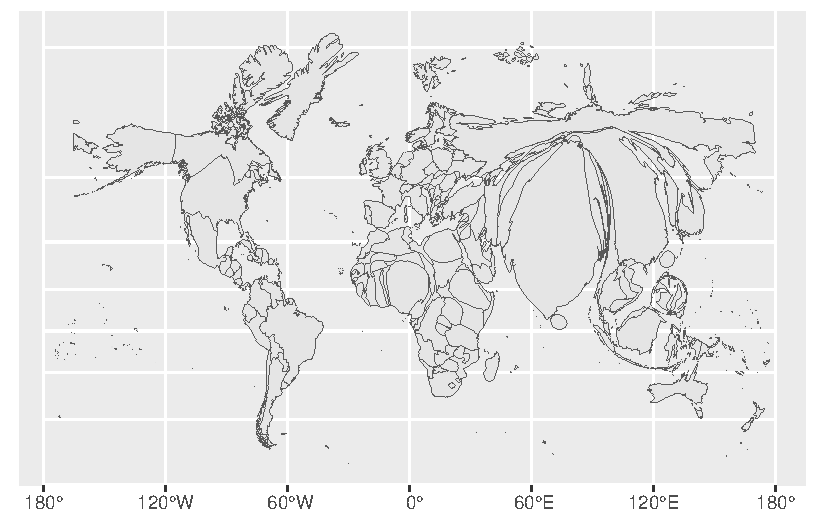
\includegraphics{cartogram_files/figure-pdf/unnamed-chunk-9-1.pdf}

\subsection{\texorpdfstring{Basic Cartogram With \texttt{fill}
Color}{Basic Cartogram With fill Color}}\label{basic-cartogram-with-fill-color}

\begin{Shaded}
\begin{Highlighting}[]
\FunctionTok{ggplot}\NormalTok{(mapdata\_cartogram) }\SpecialCharTok{+} 
  \FunctionTok{geom\_sf}\NormalTok{(}\FunctionTok{aes}\NormalTok{(}\AttributeTok{fill =}\NormalTok{ pop\_est)) }\SpecialCharTok{+} \CommentTok{\# fill is population estimate}
  \FunctionTok{theme\_void}\NormalTok{()}
\end{Highlighting}
\end{Shaded}

\includegraphics{cartogram_files/figure-pdf/unnamed-chunk-10-1.pdf}

\subsection{\texorpdfstring{Cartogram With Better (\texttt{viridis})
Colors}{Cartogram With Better (viridis) Colors}}\label{cartogram-with-better-viridis-colors}

\begin{Shaded}
\begin{Highlighting}[]
\FunctionTok{ggplot}\NormalTok{(mapdata\_cartogram) }\SpecialCharTok{+} 
  \FunctionTok{geom\_sf}\NormalTok{(}\FunctionTok{aes}\NormalTok{(}\AttributeTok{fill =}\NormalTok{ pop\_est)) }\SpecialCharTok{+} \CommentTok{\# fill is population estimate}
  \FunctionTok{scale\_fill\_viridis\_c}\NormalTok{(}\AttributeTok{name =} \StringTok{"population"}\NormalTok{,}
                       \AttributeTok{option =} \StringTok{"viridis"}\NormalTok{) }\SpecialCharTok{+} \CommentTok{\# beautiful colors}
  \FunctionTok{theme\_void}\NormalTok{()}
\end{Highlighting}
\end{Shaded}

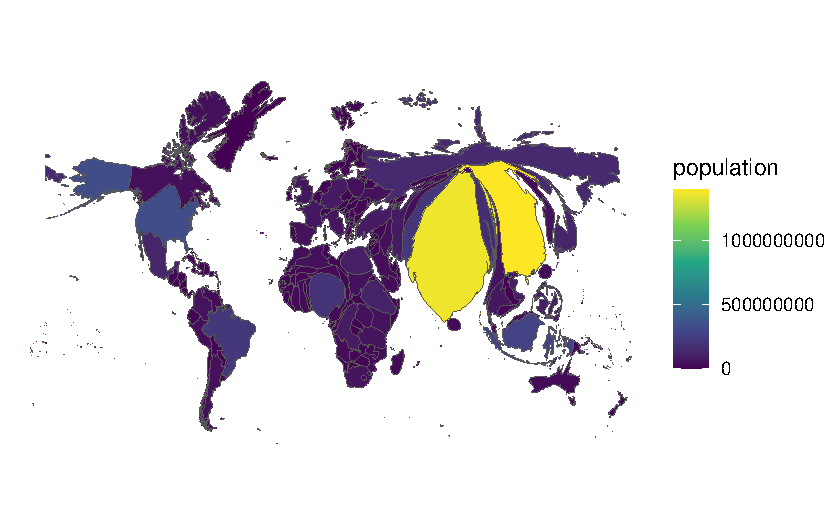
\includegraphics{cartogram_files/figure-pdf/unnamed-chunk-11-1.pdf}

\part{Other R Libraries for Mapping}

\chapter{\texorpdfstring{Mapping With
\texttt{leaflet}}{Mapping With leaflet}}\label{sec-leaflet}

\section{Call Libraries}\label{call-libraries-8}

\begin{Shaded}
\begin{Highlighting}[]
\FunctionTok{library}\NormalTok{(leaflet) }\CommentTok{\# web based maps}
\end{Highlighting}
\end{Shaded}

\begin{verbatim}
Warning: package 'leaflet' was built under R version 4.4.2
\end{verbatim}

\begin{Shaded}
\begin{Highlighting}[]
\FunctionTok{library}\NormalTok{(sf) }\CommentTok{\# simple (spatial) features}

\FunctionTok{library}\NormalTok{(readr) }\CommentTok{\# import csv}

\FunctionTok{library}\NormalTok{(dplyr) }\CommentTok{\# data wrangling}

\FunctionTok{library}\NormalTok{(here) }\CommentTok{\# where am I?}
\end{Highlighting}
\end{Shaded}

\begin{verbatim}
Warning: package 'here' was built under R version 4.4.2
\end{verbatim}

\begin{Shaded}
\begin{Highlighting}[]
\FunctionTok{library}\NormalTok{(pander) }\CommentTok{\# nice tables}

\CommentTok{\# setwd(here()) \# set the working directory}
\end{Highlighting}
\end{Shaded}

\section{Get Simulated Client Data}\label{get-simulated-client-data}

\begin{Shaded}
\begin{Highlighting}[]
\NormalTok{clients }\OtherTok{\textless{}{-}} \FunctionTok{read\_csv}\NormalTok{(}\StringTok{"./location{-}data/clients.csv"}\NormalTok{)}

\FunctionTok{pander}\NormalTok{(}\FunctionTok{head}\NormalTok{(clients)) }\CommentTok{\# top of client data}
\end{Highlighting}
\end{Shaded}

\begin{longtable}[]{@{}
  >{\centering\arraybackslash}p{(\columnwidth - 10\tabcolsep) * \real{0.0972}}
  >{\centering\arraybackslash}p{(\columnwidth - 10\tabcolsep) * \real{0.0833}}
  >{\centering\arraybackslash}p{(\columnwidth - 10\tabcolsep) * \real{0.1250}}
  >{\centering\arraybackslash}p{(\columnwidth - 10\tabcolsep) * \real{0.2639}}
  >{\centering\arraybackslash}p{(\columnwidth - 10\tabcolsep) * \real{0.2222}}
  >{\centering\arraybackslash}p{(\columnwidth - 10\tabcolsep) * \real{0.1667}}@{}}
\caption{Table continues below}\tabularnewline
\toprule\noalign{}
\begin{minipage}[b]{\linewidth}\centering
ID
\end{minipage} & \begin{minipage}[b]{\linewidth}\centering
age
\end{minipage} & \begin{minipage}[b]{\linewidth}\centering
gender
\end{minipage} & \begin{minipage}[b]{\linewidth}\centering
race\_ethnicity
\end{minipage} & \begin{minipage}[b]{\linewidth}\centering
family\_income
\end{minipage} & \begin{minipage}[b]{\linewidth}\centering
program
\end{minipage} \\
\midrule\noalign{}
\endfirsthead
\toprule\noalign{}
\begin{minipage}[b]{\linewidth}\centering
ID
\end{minipage} & \begin{minipage}[b]{\linewidth}\centering
age
\end{minipage} & \begin{minipage}[b]{\linewidth}\centering
gender
\end{minipage} & \begin{minipage}[b]{\linewidth}\centering
race\_ethnicity
\end{minipage} & \begin{minipage}[b]{\linewidth}\centering
family\_income
\end{minipage} & \begin{minipage}[b]{\linewidth}\centering
program
\end{minipage} \\
\midrule\noalign{}
\endhead
\bottomrule\noalign{}
\endlastfoot
2892 & 23 & Male & African American & 42359 & Program B \\
1971 & 39 & Female & Asian American & 66500 & Program C \\
4728 & 26 & Female & Asian American & 52726 & Program C \\
1020 & 24 & Male & Latinx & 52911 & Program D \\
4429 & 36 & Female & Asian American & 50287 & Program C \\
3136 & 33 & Male & African American & 45570 & Program C \\
\end{longtable}

\begin{longtable}[]{@{}
  >{\centering\arraybackslash}p{(\columnwidth - 6\tabcolsep) * \real{0.2639}}
  >{\centering\arraybackslash}p{(\columnwidth - 6\tabcolsep) * \real{0.2639}}
  >{\centering\arraybackslash}p{(\columnwidth - 6\tabcolsep) * \real{0.1528}}
  >{\centering\arraybackslash}p{(\columnwidth - 6\tabcolsep) * \real{0.1667}}@{}}
\toprule\noalign{}
\begin{minipage}[b]{\linewidth}\centering
mental\_health\_T1
\end{minipage} & \begin{minipage}[b]{\linewidth}\centering
mental\_health\_T2
\end{minipage} & \begin{minipage}[b]{\linewidth}\centering
latitude
\end{minipage} & \begin{minipage}[b]{\linewidth}\centering
longitude
\end{minipage} \\
\midrule\noalign{}
\endhead
\bottomrule\noalign{}
\endlastfoot
95.25 & 106.8 & 42.16 & -83.6 \\
82.64 & 96.3 & 42.29 & -83.88 \\
80.49 & 98.72 & 42.14 & -83.78 \\
93.82 & 91.67 & 42.24 & -83.68 \\
83.37 & 99.69 & 42.18 & -83.64 \\
75.28 & 92.9 & 42.21 & -83.7 \\
\end{longtable}

\section{Only Clients In Ann Arbor
Area}\label{only-clients-in-ann-arbor-area-1}

\begin{Shaded}
\begin{Highlighting}[]
\NormalTok{clients }\OtherTok{\textless{}{-}}\NormalTok{ clients }\SpecialCharTok{\%\textgreater{}\%} 
  \FunctionTok{filter}\NormalTok{(latitude }\SpecialCharTok{\textless{}=} \FloatTok{42.35} \SpecialCharTok{\&}
\NormalTok{           latitude }\SpecialCharTok{\textgreater{}=} \FloatTok{42.2} \SpecialCharTok{\&}
\NormalTok{           longitude }\SpecialCharTok{\textgreater{}=} \SpecialCharTok{{-}}\FloatTok{83.8} \SpecialCharTok{\&}
\NormalTok{           longitude }\SpecialCharTok{\textless{}=} \SpecialCharTok{{-}}\FloatTok{83.65}\NormalTok{)}
\end{Highlighting}
\end{Shaded}

\section{Read in Shapefiles}\label{read-in-shapefiles-1}

\begin{Shaded}
\begin{Highlighting}[]
\NormalTok{parks }\OtherTok{\textless{}{-}} \FunctionTok{read\_sf}\NormalTok{(}\StringTok{"./shapefiles/AA\_Parks/AA\_Parks.shp"}\NormalTok{)}

\NormalTok{university }\OtherTok{\textless{}{-}} \FunctionTok{read\_sf}\NormalTok{(}\StringTok{"./shapefiles/AA\_University/AA\_University.shp"}\NormalTok{)}

\NormalTok{city\_boundary }\OtherTok{\textless{}{-}} \FunctionTok{read\_sf}\NormalTok{(}\StringTok{"./shapefiles/AA\_City\_Boundary/AA\_City\_Boundary.shp"}\NormalTok{)}
\end{Highlighting}
\end{Shaded}

\chapter{Transform CRS}\label{transform-crs}

\begin{quote}
``Map projections try to portray the surface of the earth or a portion
of the earth on a flat piece of paper or computer screen. A coordinate
reference system (CRS) then defines, with the help of coordinates, how
the two-dimensional, projected map in your GIS is related to real places
on the earth. The decision as to which map projection and coordinate
reference system to use, depends on the regional extent of the area you
want to work in, on the analysis you want to do and often on the
availability of data.'' From
\href{https://docs.qgis.org/2.8/en/docs/gentle_gis_introduction/coordinate_reference_systems.html}{qgis.org}
\end{quote}

\begin{quote}
see
\url{https://stackoverflow.com/questions/66471147/how-to-plot-sp-object-as-sf-in-r-leaflet}
\end{quote}

\begin{Shaded}
\begin{Highlighting}[]
\NormalTok{university }\OtherTok{\textless{}{-}} \FunctionTok{st\_transform}\NormalTok{(university, }\DecValTok{4326}\NormalTok{) }\CommentTok{\# transform CRS}

\NormalTok{parks }\OtherTok{\textless{}{-}} \FunctionTok{st\_transform}\NormalTok{(parks, }\DecValTok{4326}\NormalTok{) }\CommentTok{\# transform CRS}

\NormalTok{city\_boundary }\OtherTok{\textless{}{-}} \FunctionTok{st\_transform}\NormalTok{(city\_boundary, }\DecValTok{4326}\NormalTok{) }\CommentTok{\# transform CRS}
\end{Highlighting}
\end{Shaded}

\section{Leaflet Map}\label{leaflet-map}

\subsection{Color Palette}\label{color-palette}

\begin{Shaded}
\begin{Highlighting}[]
\NormalTok{pal }\OtherTok{\textless{}{-}} \FunctionTok{colorFactor}\NormalTok{(}\FunctionTok{c}\NormalTok{(}\StringTok{"red"}\NormalTok{, }\StringTok{"blue"}\NormalTok{, }\StringTok{"orange"}\NormalTok{, }\StringTok{"green"}\NormalTok{), }
                   \AttributeTok{domain =} \FunctionTok{levels}\NormalTok{(}\FunctionTok{as.factor}\NormalTok{(clients}\SpecialCharTok{$}\NormalTok{program)))}
\end{Highlighting}
\end{Shaded}

\subsection{Map}\label{map-2}

\begin{Shaded}
\begin{Highlighting}[]
\FunctionTok{leaflet}\NormalTok{(clients) }\SpecialCharTok{\%\textgreater{}\%}
  \FunctionTok{setView}\NormalTok{(}\AttributeTok{lng =} \FunctionTok{mean}\NormalTok{(clients}\SpecialCharTok{$}\NormalTok{longitude), }
          \AttributeTok{lat =} \FunctionTok{mean}\NormalTok{(clients}\SpecialCharTok{$}\NormalTok{latitude), }
          \AttributeTok{zoom =} \DecValTok{12}\NormalTok{) }\SpecialCharTok{\%\textgreater{}\%} 
  \CommentTok{\# addTiles() \%\textgreater{}\% \# Open StreetMap}
  \FunctionTok{addProviderTiles}\NormalTok{(providers}\SpecialCharTok{$}\NormalTok{CartoDB.Positron) }\SpecialCharTok{\%\textgreater{}\%}
  \FunctionTok{addCircleMarkers}\NormalTok{(}\SpecialCharTok{\textasciitilde{}}\NormalTok{longitude, }
             \SpecialCharTok{\textasciitilde{}}\NormalTok{latitude, }
             \AttributeTok{popup =} \SpecialCharTok{\textasciitilde{}}\FunctionTok{paste}\NormalTok{(}\StringTok{"Client ID:"}\NormalTok{, }\FunctionTok{as.character}\NormalTok{(ID)), }
             \AttributeTok{label =} \SpecialCharTok{\textasciitilde{}}\FunctionTok{paste}\NormalTok{(}\StringTok{"Client ID:"}\NormalTok{, }\FunctionTok{as.character}\NormalTok{(ID)),}
             \AttributeTok{color =} \SpecialCharTok{\textasciitilde{}}\FunctionTok{pal}\NormalTok{(program),}
             \AttributeTok{clusterOptions =} \FunctionTok{markerClusterOptions}\NormalTok{()) }\SpecialCharTok{\%\textgreater{}\%}
  \FunctionTok{addLegend}\NormalTok{(}\StringTok{"bottomright"}\NormalTok{, }
            \AttributeTok{pal =}\NormalTok{ pal, }
            \AttributeTok{values =} \SpecialCharTok{\textasciitilde{}}\NormalTok{program,}
            \AttributeTok{title =} \StringTok{"Program"}\NormalTok{) }\SpecialCharTok{\%\textgreater{}\%}
  \CommentTok{\# addPolygons(data = parks, color = "green") \%\textgreater{}\%}
  \CommentTok{\# addPolygons(data = university, color = "blue") \%\textgreater{}\%}
  \FunctionTok{addPolygons}\NormalTok{(}\AttributeTok{data =}\NormalTok{ city\_boundary, }
              \AttributeTok{color =} \StringTok{"red"}\NormalTok{,}
              \AttributeTok{fillOpacity =} \FloatTok{0.0}\NormalTok{)}
\end{Highlighting}
\end{Shaded}

\includegraphics{leaflet_files/figure-pdf/unnamed-chunk-7-1.pdf}

\chapter{\texorpdfstring{Mapping With
\texttt{plotly}}{Mapping With plotly}}\label{mapping-with-plotly}

\section{Call Libraries}\label{call-libraries-9}

\begin{Shaded}
\begin{Highlighting}[]
\FunctionTok{library}\NormalTok{(plotly)}
\end{Highlighting}
\end{Shaded}

\begin{verbatim}
Warning: package 'plotly' was built under R version 4.4.2
\end{verbatim}

\section{Set Geographic Parameters}\label{set-geographic-parameters}

\begin{Shaded}
\begin{Highlighting}[]
\NormalTok{g }\OtherTok{\textless{}{-}} \FunctionTok{list}\NormalTok{(}\AttributeTok{showland =} \ConstantTok{TRUE}\NormalTok{, }
          \AttributeTok{showcountries =} \ConstantTok{TRUE}\NormalTok{,}
          \AttributeTok{landcolor =} \FunctionTok{toRGB}\NormalTok{(}\StringTok{"forestgreen"}\NormalTok{), }\CommentTok{\# land color}
          \AttributeTok{showocean =} \ConstantTok{TRUE}\NormalTok{, }\CommentTok{\# show ocean}
          \AttributeTok{oceancolor =} \StringTok{"lightblue"}\NormalTok{, }\CommentTok{\# ocean color}
          \CommentTok{\# projection = list(type = \textquotesingle{}robinson\textquotesingle{}),}
          \AttributeTok{projection =} \FunctionTok{list}\NormalTok{(}\AttributeTok{type =} \StringTok{\textquotesingle{}orthographic\textquotesingle{}}\NormalTok{,}
                    \AttributeTok{rotation =} \FunctionTok{list}\NormalTok{(}\AttributeTok{lon =} \DecValTok{0}\NormalTok{,}
                                    \AttributeTok{lat =} \DecValTok{0}\NormalTok{,}
                                    \AttributeTok{roll =} \DecValTok{0}\NormalTok{)))}
\end{Highlighting}
\end{Shaded}

\section{Make a Map}\label{make-a-map}

\begin{Shaded}
\begin{Highlighting}[]
\FunctionTok{plot\_geo}\NormalTok{() }\SpecialCharTok{\%\textgreater{}\%} 
  \FunctionTok{layout}\NormalTok{(}\AttributeTok{title =} \StringTok{"Demonstration Map"}\NormalTok{, }
         \AttributeTok{geo =}\NormalTok{ g)}
\end{Highlighting}
\end{Shaded}

\includegraphics{plotly_files/figure-pdf/unnamed-chunk-3-1.pdf}

\section{\texorpdfstring{\texttt{scattermapbox}}{scattermapbox}}\label{scattermapbox}

\begin{Shaded}
\begin{Highlighting}[]
\FunctionTok{plot\_ly}\NormalTok{(}\AttributeTok{type =} \StringTok{"scattermapbox"}\NormalTok{) }\SpecialCharTok{\%\textgreater{}\%}
  \FunctionTok{layout}\NormalTok{(}
    \AttributeTok{mapbox =} \FunctionTok{list}\NormalTok{(}
      \AttributeTok{style =} \StringTok{\textquotesingle{}open{-}street{-}map\textquotesingle{}}\NormalTok{,}
      \AttributeTok{zoom =} \FloatTok{6.0}\NormalTok{, }\CommentTok{\# zoom}
      \AttributeTok{center =} \FunctionTok{list}\NormalTok{(}\AttributeTok{lon =} \SpecialCharTok{{-}}\DecValTok{83}\NormalTok{, }\AttributeTok{lat =} \DecValTok{42}\NormalTok{))) }\CommentTok{\# centered on SE Michigan}
\end{Highlighting}
\end{Shaded}

\includegraphics{plotly_files/figure-pdf/unnamed-chunk-4-1.pdf}




\end{document}
